% +------------------------------------------------------------------------+
% | CGAL Reference Manual:  polyhedron.tex
% +------------------------------------------------------------------------+
% | Combinatoric and geometry of polyhedral surfaces in 
% | halfedge representation.
% |
% | 11.10.1996   Lutz Kettner
% |              Start rewriting the whole stuff
% | 
\RCSdef{\polyhedronRev}{$Id$}
\RCSdefDate{\polyhedronDate}{$Date$}
% +------------------------------------------------------------------------+

\ccParDims

\ccUserChapter{3D Polyhedral Surfaces \label{chapterPolyhedron}}

\ccChapterRelease{\polyhedronRev. \ \polyhedronDate}
\ccChapterAuthor{Lutz Kettner}



\begin{ccPkgDescription}{3D Convex Hulls\label{Pkg:ConvexHull3}}
\ccPkgHowToCiteCgal{cgal:hs-ch3-07}
\ccPkgSummary{This package provides functions 
for computing convex hulls in three dimensions as well as functions
for checking if sets of points are strongly convex are not. One can
compute the convex hull of a set of points in three dimensions in one
of three ways: using a static algorithm, using an incremental
construction algorithm, or using a triangulation to get a fully
dynamic computation.}

\ccPkgDependsOn{All algorithms produce as output a \ccRef[3D Polyhedron]{Pkg:Polyhedron}. 
                The dynamic algorithms depend on \ccRef[3D Triangulations]{Pkg:Triangulation3}}
\ccPkgIntroducedInCGAL{1.1}
\ccPkgLicense{\ccLicenseQPL}
\ccPkgIllustration{Convex_hull_3/bunny.png}{Convex_hull_3/bunny.png}
\end{ccPkgDescription}


\begin{ccTexOnly}
    \setlength{\unitlength}{1mm}
    \begin{picture}(0,0)(0.0,0.0)
      \put (78,25){% textwidth = 156mm
          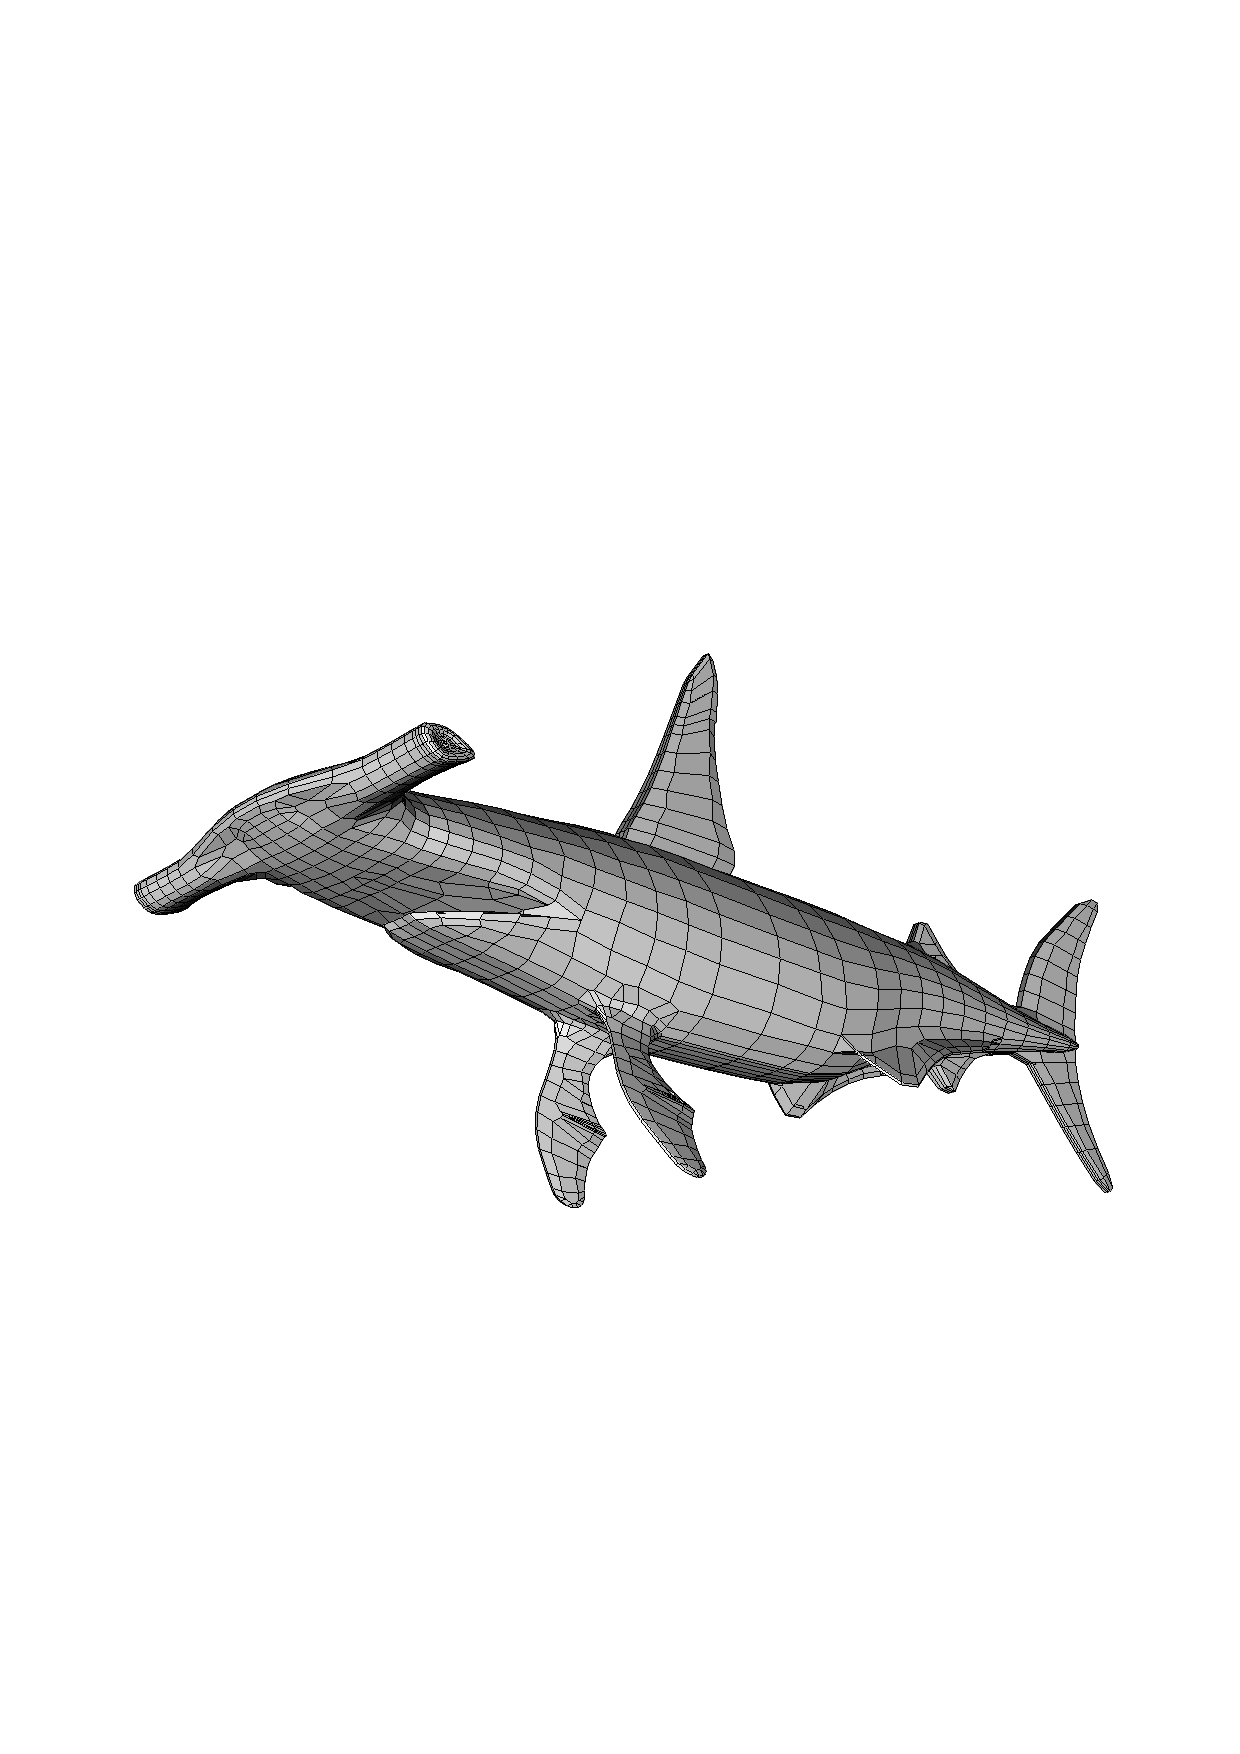
\includegraphics[width=0.5\textwidth]{Polyhedron/fig/shark}
      }
    \end{picture}\vspace{-4mm}% compensate for some vspace added by picture
\end{ccTexOnly}

\minitoc

% +------------------------------------------------------------------------+
\section{Introduction\label{sectionPolyIntro}}

% \begin{ccTexOnly}
%     \vspace*{-50mm}
%     \begin{flushright}~\hspace{1cm}
%       \parbox{0.5\textwidth}{%
%           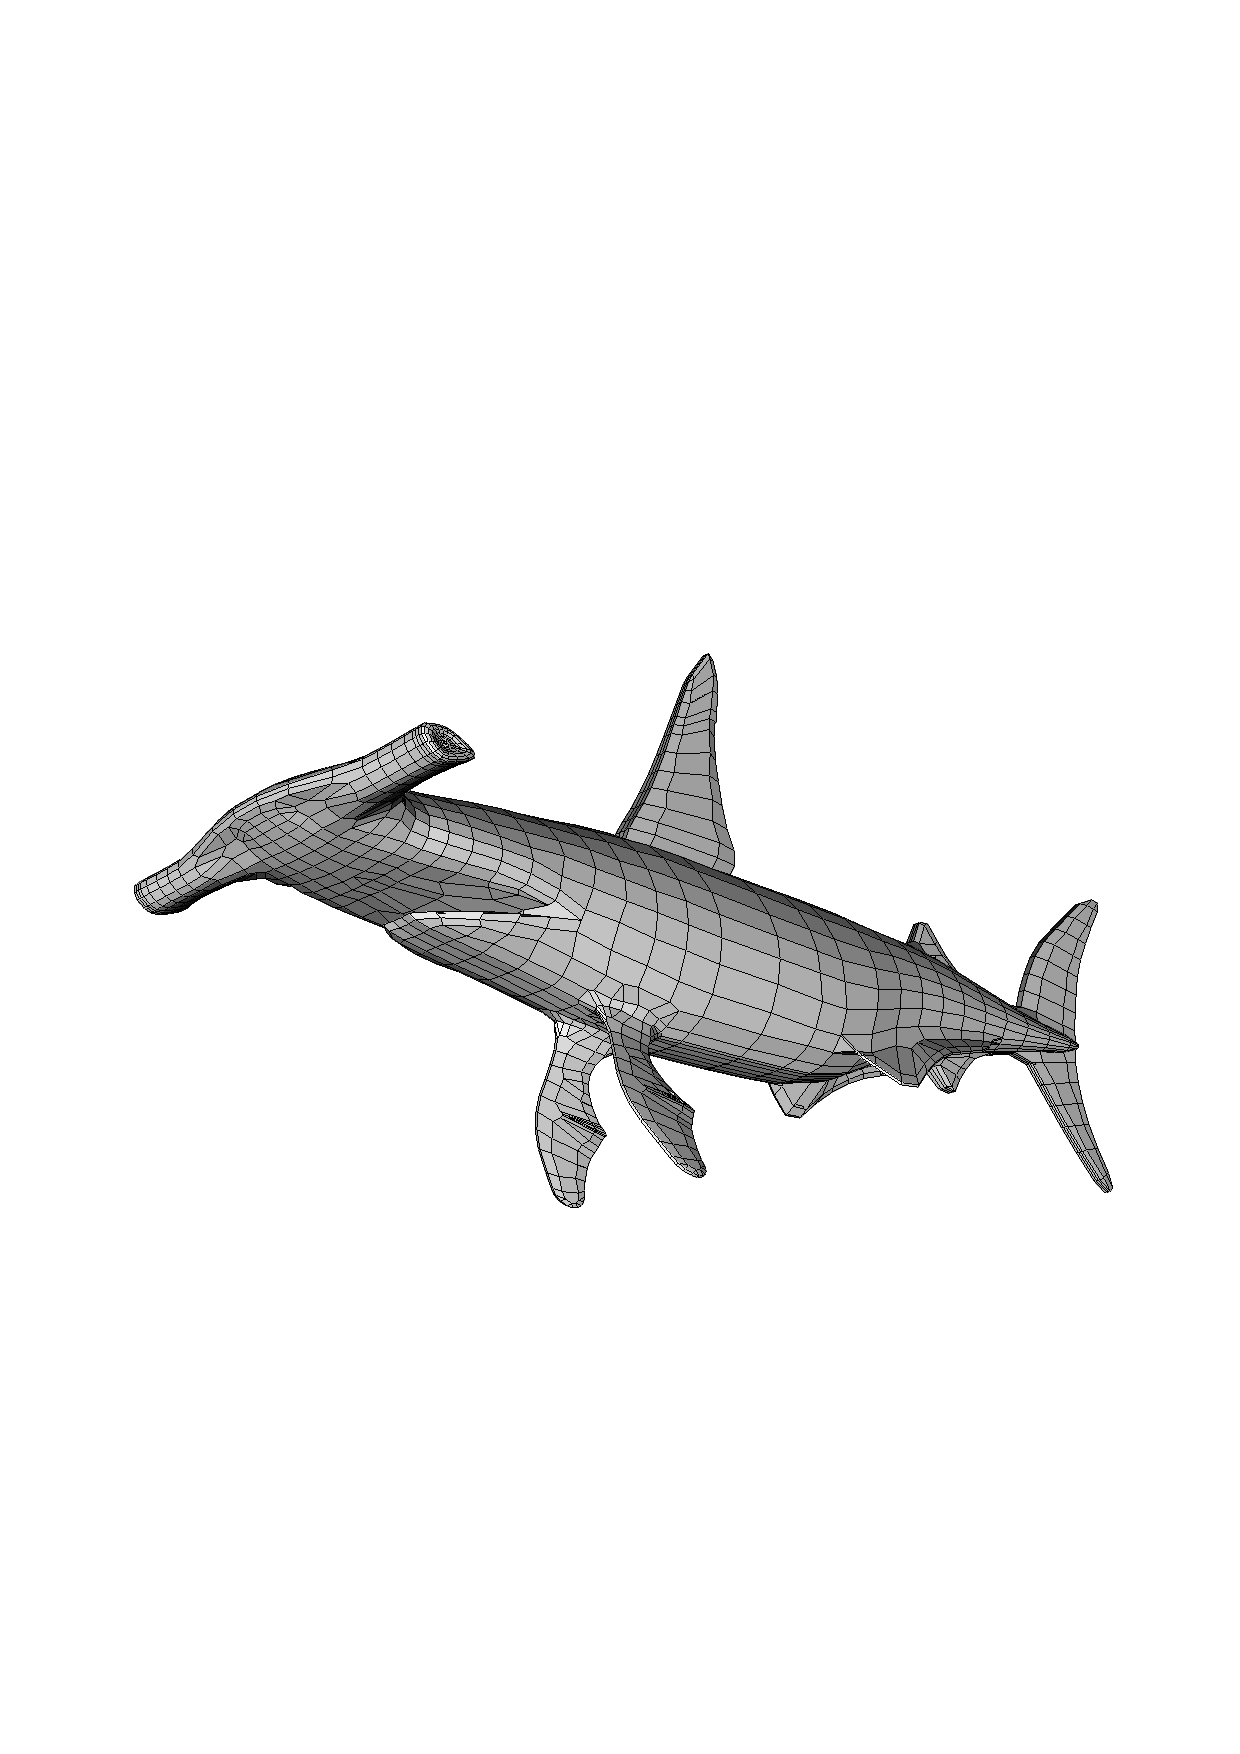
\includegraphics[width=0.5\textwidth]{Polyhedron/fig/shark}%
%       }%
%     \end{flushright}
% \end{ccTexOnly}

Polyhedral surfaces in three dimensions are composed of vertices,
edges, facets and an incidence relationship on them. The organization
beneath is a halfedge data structure, which restricts the class of
representable surfaces to orientable 2-manifolds -- with and without
boundary. If the surface is closed we call it a {\em polyhedron}, for
example, see the \ccTexHtml{above}{following} model of a hammerhead:

\begin{ccHtmlOnly}
    <CENTER>
        <img src="./fig/shark.gif" alt="Hammerhead"><P>
    </CENTER>
\end{ccHtmlOnly}

The polyhedral surface is realized as a container class that manages
vertices, halfedges, facets with their incidences, and that maintains
the combinatorial integrity of them. It is based on the highly
flexible design of the halfedge data structure, see the introduction
in Chapter~\ref{chapterHalfedgeDS} and~\cite{k-ugpdd-99}. However, the
polyhedral surface can be used and understood without knowing the
underlying design. Some of the examples in this chapter introduce also
gradually into first applications of this flexibility.

% +========================================================================+
\section{Definition}
% +========================================================================+
  
A polyhedral surface \ccc{CGAL::Polyhedron_3<PolyhedronTraits_3>} in
three dimensions consists of vertices $V$, edges $E$, facets $F$ and
an incidence relation on them.  Each edge is represented by two
halfedges with opposite orientations. The incidences stored with a
halfedge are illustrated in the following figure:

\begin{ccTexOnly}
    \vspace{-7mm}
    \begin{center}
      \parbox{0.4\textwidth}{%
          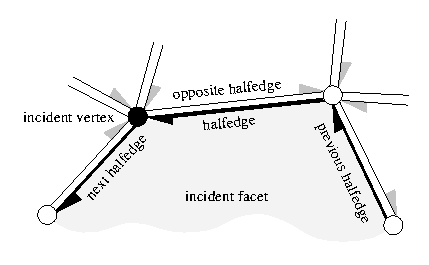
\includegraphics[width=0.4\textwidth]{Polyhedron/fig/halfedge}%
      }
    \end{center}
    \vspace{-5mm}
\end{ccTexOnly}

\begin{ccHtmlOnly}
    <CENTER>
    <A HREF="./fig/halfedge.gif">
        <img src="./fig/halfedge_small.gif" alt="Halfedge Diagram"></A><P>
    </CENTER>
\end{ccHtmlOnly}

Vertices represent points in space. Edges are straight line segments
between two endpoints. Facets are planar polygons without
holes. Facets are defined by the circular sequence of halfedges along
their boundary.  The polyhedral surface itself can have holes (with at
least two facets surrounding it since a single facet cannot have a
hole). The halfedges along the boundary of a hole are called {\em
border halfedges\/} and have no incident facet. An edge is a {\em
border edge\/} if one of its halfedges is a border halfedge.  A
surface is {\em closed\/} if it contains no border halfedges. A closed
surface is a boundary representation for polyhedra in three
dimensions. The convention is that the halfedges are oriented
counterclockwise around facets as seen from the outside of the
polyhedron. An implication is that the halfedges are oriented
clockwise around the vertices. The notion of the solid side of a facet
as defined by the halfedge orientation extends to polyhedral surfaces
with border edges although they do not define a closed object. If
normal vectors are considered for the facets, normals point outwards
(following the right-hand rule).

The strict definition can be found in~\cite{k-ugpdd-99}. One
implication of this definition is that the polyhedral surface is
always an orientable and oriented 2-manifold with border edges, i.e.,
the neighborhood of each point on the polyhedral surface is either
homeomorphic to a disc or to a half disc, except for vertices where
many holes and surfaces with boundary can join. Another implication is
that the smallest representable surface avoiding self intersections is
a triangle (for polyhedral surfaces with border edges) or a
tetrahedron (for polyhedra). Boundary representations of orientable
2-manifolds are closed under Euler operations. They are extended with
operations that create or close holes in the surface.

Other intersections besides the incidence relation are not allowed.
However, this is not automatically verified in the operations, since
self intersections are not easy to check
efficiently. \ccc{CGAL::Polyhedron_3<PolyhedronTraits_3>} does only
maintain the combinatorial integrity of the polyhedral surface (using
Euler operations) and does not consider the coordinates of the points
or any other geometric information.

\ccc{CGAL::Polyhedron_3<PolyhedronTraits_3>} can represent polyhedral
surfaces as well as polyhedra. The interface is designed in such a way
that it is easy to ignore border edges and work only with polyhedra.


% +========================================================================+
\section{Example Programs}
% +========================================================================+
\label{sectionPolyExamples}

The polyhedral surface is based on the highly flexible design of the
halfedge data structure. Examples for this flexibility can be found in
Section~\ref{sectionPolyExtend} and in Section~\ref{sectionHdsExamples}. 
This design is not a prerequisite to understand the following examples.
See also the Section~\ref{sectionPolyAdvanced} below for some advanced 
examples.

% +-------------------------------------------------------------+
\subsection{First Example Using Defaults}

The first example instantiates a polyhedron using a kernel as traits
class. It creates a tetrahedron and stores the reference to one of its
halfedges in a \ccc{Halfedge_handle}. Handles, also know as
{\em trivial iterators}, are used to keep references to halfedges,
vertices, or facets for future use. There is also a \ccc{Halfedge_iterator}
type for enumerating halfedges. Such an iterator type can be used 
wherever a handle is required. Respective \ccc{Halfedge_const_handle} and
\ccc{Halfedge_const_iterator} for a constant polyhedron and similar
handles and iterators with \ccc{Vertex_} and \ccc{Facet_} prefix
are provided too.

The example continues with a test if the halfedge
actually refers to a tetrahedron. This test checks the connected 
component referred to by the halfedge \ccc{h} and not the polyhedral
surface as a whole. This examples works only on the combinatorial
level of a polyhedral surface. The next example adds the geometry.

\ccIncludeExampleCode{Polyhedron/polyhedron_prog_simple.cpp}

% +-------------------------------------------------------------+
\subsection{Example with Geometry in Vertices}

We add geometry to the our construction of a tetrahedron. Four points
are passed as arguments to the construction. This example demonstrates
in addition the use of the vertex iterator and the access to the point
in the vertices. Note the natural access notation \ccc{v->point()}.
Similarly, all information stored in a vertex, halfedge, and facet can
be accessed with a member function given a handle or iterator. For
example, given a halfedge handle \ccc{h} we can write \ccc{h->next()}
to get a halfedge handle to the next halfedge, \ccc{h->opposite()} for
the opposite halfedge, \ccc{h->vertex()} for the incident vertex at
the tip of \ccc{h}, and so on.  The output of the program will be
"\verb|1 0 0\n0 1 0\n0 0 1\n0 0 0\n|".

%\newpage
\ccIncludeExampleCode{Polyhedron/polyhedron_prog_tetra.cpp}

The polyhedron offers a point iterator for convenience. The above
\texttt{for} loop simplifies to a single statement by using
\ccc{std::copy} and the ostream iterator adaptor.

\begin{ccExampleCode}
std::copy( P.points_begin(), P.points_end(), 
           std::ostream_iterator<Point_3>(std::cout,"\n"));
\end{ccExampleCode}

% +-------------------------------------------------------------+
\subsection{Example for Affine Transformation}

An affine transformation $A$ can act as a functor transforming points
and a point iterator is conveniently defined for polyhedral surfaces.
So, assuming we want only the point coordinates of a polyhedron $P$
transformed, \ccc{std::transform} does the job in a single line.

\begin{ccExampleCode}
std::transform( P.points_begin(), P.points_end(), P.points_begin(), A);
\end{ccExampleCode}


% +-------------------------------------------------------------+
\subsection{Example Computing Plane Equations}

The polyhedral surface has already provisions to store a plane
equation for each facet. However, it does not provide a function to
compute plane equations.

This example computes the plane equations of a polyhedral surface.
The actual computation is implemented in the
\texttt{compute\_plane\_equations} function.  Depending on the arithmetic
(exact/inexact) and the shape of the facets (convex/non-convex)
different methods are useful. We assume here strictly convex facets
and exact arithmetic. In our example a homogeneous representation with
\texttt{int} coordinates is sufficient. The four plane equations of the
tetrahedron are the output of the program.

\ccIncludeExampleCode{Polyhedron/polyhedron_prog_planes.cpp}

% +-------------------------------------------------------------+
\subsection{Example with a Vector Instead of a List Representation\label{sectionPolyVector}}

The polyhedron class template has actually four parameters, where
three of them have default values. Using the default values explicitly
in our examples above for three parameter---ignoring the fourth
parameter, which would be a standard allocator for container class---
the definition of a polyhedron looks like:

\begin{ccExampleCode}
typedef CGAL::Polyhedron_3< Traits, 
                            CGAL::Polyhedron_items_3, 
                            CGAL::HalfedgeDS_default>      Polyhedron;
\end{ccExampleCode}

The \ccc{CGAL::Polyhedron_items_3} class contains the types used for
vertices, edges, and facets. The \ccc{CGAL::HalfedgeDS_default} class
defines the halfedge data structure used, which is a list-based
representation in this case. An alternative is a vector-based
representation. Using a vector provides random
access for the elements in the polyhedral surface and is more space
efficient, but elements cannot be deleted arbitrarily. Using a list
allows arbitrary deletions, but provides only bidirectional iterators
and is less space efficient. The following example creates again a 
tetrahedron with given points, but in a vector-based representation.

The vector-based representation resizes automatically if the reserved
capacity is not sufficient for the new items created. Upon resizing
all handles, iterators, and circulators become invalid. Their correct
update in the halfedge data structure is costly, thus it is advisable
to reserve enough space in advance as indicated with the alternative
constructor in the comment. 

\begin{ccAdvanced}
Note that the polyhedron and not the underlying halfedge data
structure triggers the resize operation, since the resize operation
requires some preconditions, such as valid incidences, to be fulfilled
that only the polyhedron can guarantee.
\end{ccAdvanced}

\ccIncludeExampleCode{Polyhedron/polyhedron_prog_vector.cpp}


% +-------------------------------------------------------------+
\subsection{Example with Circulator Writing Object File Format (OFF)}

We create a tetrahedron and write it to \ccc{std::cout} using the
Object File Format (OFF)~\cite{cgal:p-gmgv16-96}.  This example makes use
of \stl\ algorithms (\ccc{std::copy}, \ccc{std::distance}), \stl\
\ccc{std::ostream_iterator}, and \cgal\ circulators. The polyhedral
surface provides convenient circulators for the counterclockwise
circular sequence of halfedges around a facet and the clockwise
circular sequence of halfedges around a vertex.

However, the computation of the vertex index in the inner loop of the
facet output is not advisable with the \ccc{std::distance} function,
since it takes linear time for non random-access iterators, which
leads to quadratic runtime. For better runtime the vertex index needs
to be stored separately and computed once before writing the
facets. It can be stored, for example, in the vertex itself or in a
hash-structure.  See also the following Section~\ref{sectionPolyIO} for 
file I/O.

\ccIncludeExampleCode{Polyhedron/polyhedron_prog_off.cpp}

% +-------------------------------------------------------------+
\subsection{Example Using Euler Operators to Build a Cube}

Euler operators are the natural way of modifying polyhedral surfaces.
We provide a set of operations for polyhedra: \ccc{split_facet()}, 
\ccc{join_facet()}, \ccc{split_vertex()}, \ccc{join_vertex()},
\ccc{split_loop()}, and \ccc{join_loop()}. We add further convenient
operators, such as \ccc{split_edge()}. However, they could be implemented 
using the six operators above. Furthermore, we provide more operators
to work with polyhedral surfaces with border edges, for example, creating
and deleting holes. We refer to the references manual for the 
definition and illustrative figures of the Euler operators.

The following example implements a function that appends a unit cube
to a polyhedral surface. To keep track of the different steps during
the creation of the cube a sequence of sketches might help with labels
for the different handles that occur in the program code. The following
Figure shows six selected steps from the creation sequence. These steps 
are also marked in the program code.

\begin{ccTexOnly}
    \begin{center}
      \parbox{\textwidth}{%
          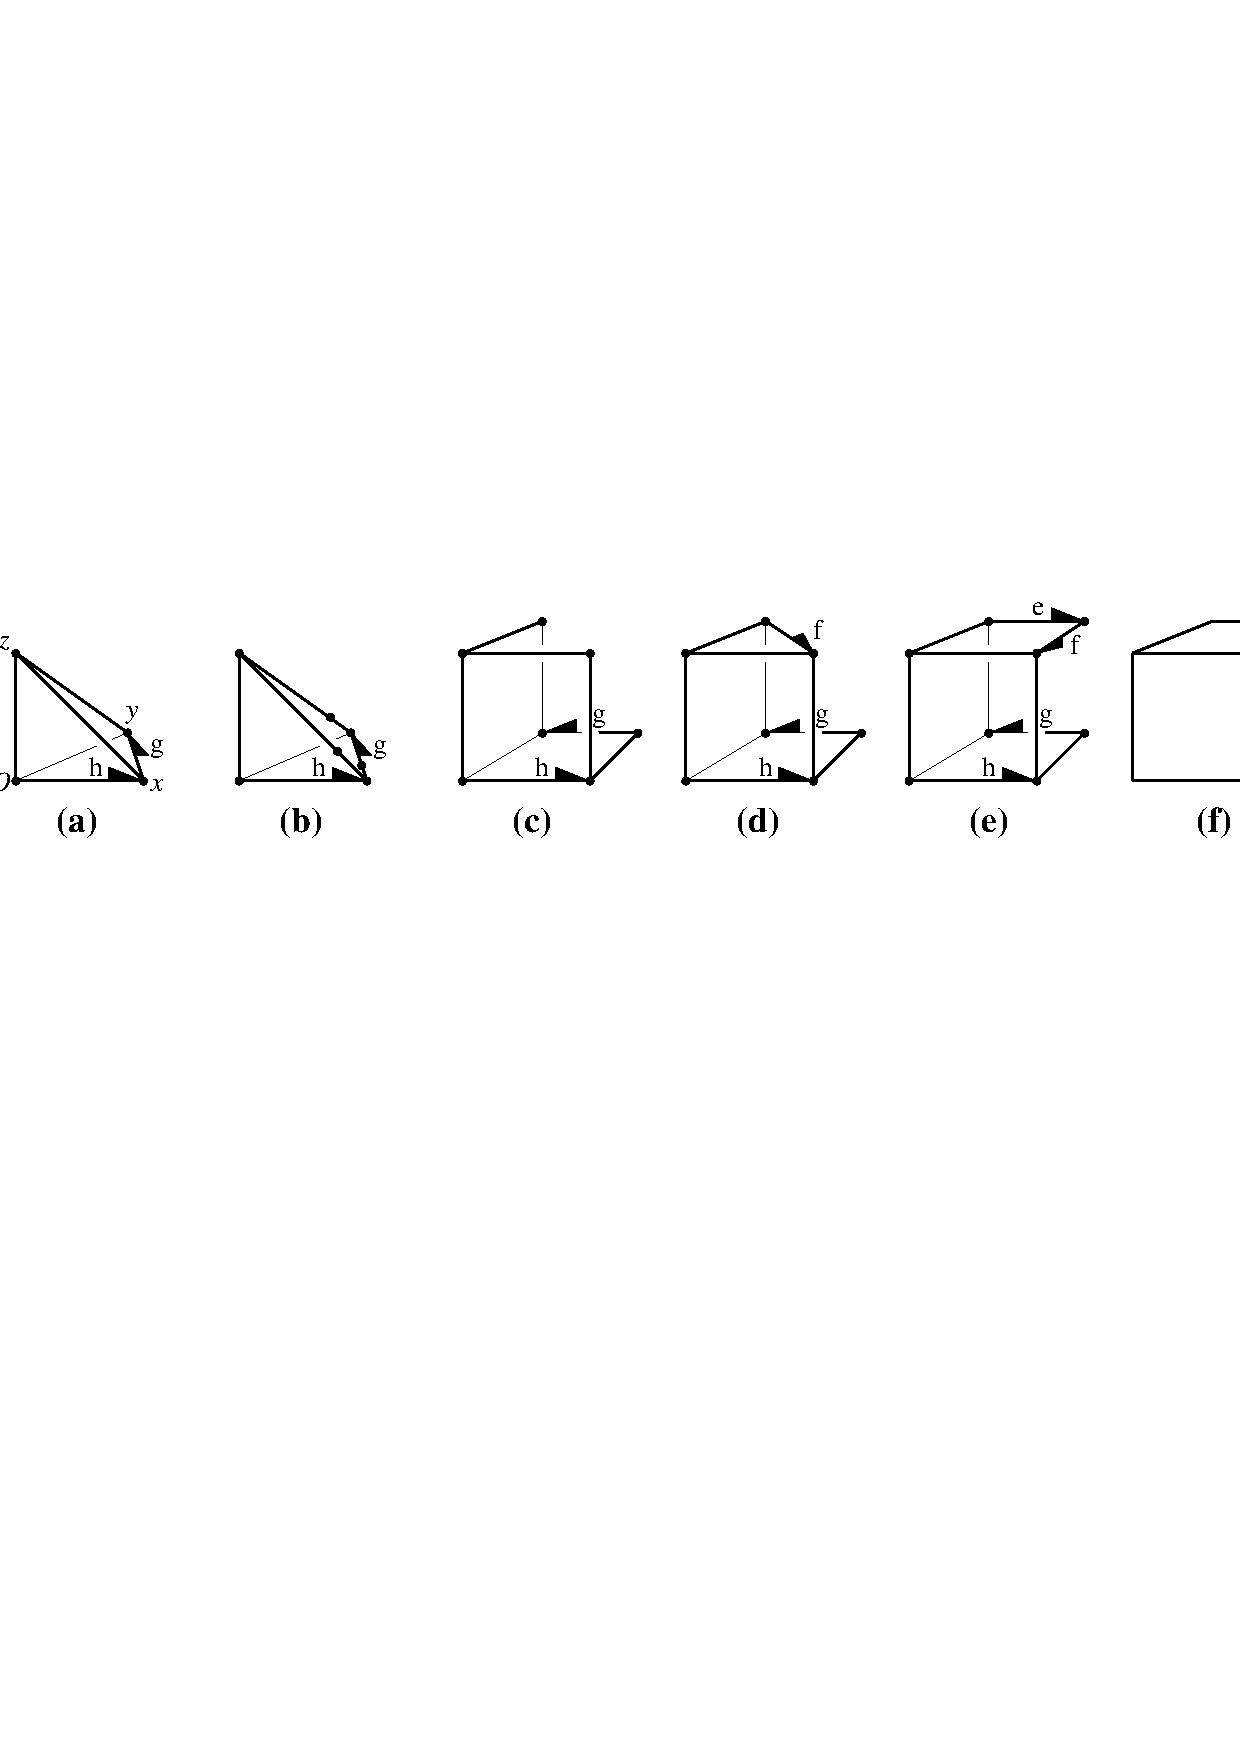
\includegraphics[width=\textwidth]{Polyhedron/fig/make_cube}%
      }
    \end{center}
\end{ccTexOnly}

\begin{ccHtmlOnly}
    <CENTER>
        <img src="./fig/make_cube.gif" alt="Steps in making a cube."><P>
    </CENTER>
\end{ccHtmlOnly}


\ccIncludeExampleCode{Polyhedron/polyhedron_prog_cube.cpp}



% +========================================================================+
\section{File I/O}
% +========================================================================+
\label{sectionPolyIO}

Simple file I/O for polyhedral surfaces is already provided in the
library. The file I/O considers so far only the topology of the
surface and its point coordinates. It ignores a possible plane
equation or any user-added attributes, such as color.

The default file format supported in \cgal\ for output as well as for
input is the Object File Format, OFF, with file extension {\tt .off},
which is also understood by Geomview~\cite{cgal:p-gmgv16-96}. For OFF
an ASCII and a binary format exist. The format can be selected with
the \cgal\ modifiers for streams, \ccc{set_ascii_mode} and
\ccc{set_binary_mode} respectively. The modifier \ccc{set_pretty_mode}
can be used to allow for (a few) structuring comments in the
output. Otherwise, the output would be free of comments.  The default
for writing is ASCII without comments. Both, ASCII and binary format,
can be read independent of the stream setting. Since this file format
is the default format, iostream operators are provided for it.

\ccThree{Inventor_ostream&M}{}{.}
\ccInclude{CGAL/IO/Polyhedron_iostream.h}

\ccHtmlNoLinks
\ccGlobalFunction{template <class PolyhedronTraits_3>
    ostream& operator<<( ostream& out, 
                         const CGAL::Polyhedron_3<PolyhedronTraits_3>& P);}

\ccHtmlNoLinks
\ccGlobalFunction{template <class PolyhedronTraits_3>
    istream& operator>>( istream& in, 
                         CGAL::Polyhedron_3<PolyhedronTraits_3>& P);}


Additional formats supported for writing are OpenInventor ({\tt .iv})
\cite{cgal:w-impoo-94}, VRML 1.0 and 2.0 ({\tt .wrl})
\cite{cgal:bpp-vrml-95,cgal:vrmls-96,cgal:hw-vrml2h-96}, and Wavefront Advanced
Visualizer object format ({\tt .obj}). Another convenient output
function writes a polyhedral surface to a Geomview process spawned
from the \cgal\ program.  These output functions are provided as
stream operators, now acting on the stream type of the respective
format.

\ccInclude{CGAL/IO/Polyhedron_inventor_ostream.h}
\\
\ccInclude{CGAL/IO/Polyhedron_VRML_1_ostream.h}
\\
\ccInclude{CGAL/IO/Polyhedron_VRML_2_ostream.h}
\\
\ccInclude{CGAL/IO/Polyhedron_geomview_ostream.h}

\ccHtmlNoLinks
\ccGlobalFunction{template <class PolyhedronTraits_3>
    Inventor_ostream& operator<<( Inventor_ostream& out, 
                           const CGAL::Polyhedron_3<PolyhedronTraits_3>& P);}

\ccHtmlNoLinks
\ccGlobalFunction{template <class PolyhedronTraits_3>
    VRML_1_ostream& operator<<( VRML_1_ostream& out, 
                           const CGAL::Polyhedron_3<PolyhedronTraits_3>& P);}

\ccHtmlNoLinks
\ccGlobalFunction{template <class PolyhedronTraits_3>
    VRML_2_ostream& operator<<( VRML_2_ostream& out, 
                           const CGAL::Polyhedron_3<PolyhedronTraits_3>& P);}

\ccHtmlNoLinks
\ccGlobalFunction{template <class PolyhedronTraits_3>
    Geomview_stream& operator<<( Geomview_stream& out, 
                           const CGAL::Polyhedron_3<PolyhedronTraits_3>& P);}


All these file formats have in common that they represent a surface as
a set of facets. Each facet is a list of indices pointing into a set
of vertices. Vertices are represented as coordinate triples. The
file I/O for polyhedral surfaces \ccc{CGAL::Polyhedron_3} imposes certain 
restrictions on these formats. They must represent a permissible 
polyhedral surface, e.g., a 2-manifold and no isolated vertices, see 
Section~\ref{sectionPolyIntro}.

Some example programs around the different file formats are provided
in the distribution under \texttt{examples/Polyhedron\_IO/} and
\texttt{demo/Polyhedron\_IO/}. We show an example converting OFF input
into VRML 1.0 output.

\begin{ccExampleCode}
// examples/Polyhedron_IO/polyhedron2vrml.cpp
// ----------------------------------------

#include <CGAL/Simple_cartesian.h>
#include <CGAL/Polyhedron_3.h>
#include <CGAL/IO/Polyhedron_iostream.h>
#include <CGAL/IO/Polyhedron_VRML_1_ostream.h> 
#include <iostream>

typedef CGAL::Simple_cartesian<double> Kernel;
typedef CGAL::Polyhedron_3<Kernel>     Polyhedron;

int main() {
    Polyhedron P;
    std::cin >> P;
    CGAL::VRML_1_ostream out( std::cout);
    out << P;
    return ( std::cin && std::cout) ? 0 : 1;
}
\end{ccExampleCode}



% +========================================================================+
\section{Extending Vertices, Halfedges, and Facets}
% +========================================================================+
\label{sectionPolyExtend}

In Section~\ref{sectionPolyVector} we have seen how to change the 
default list representation

\begin{ccExampleCode}
typedef CGAL::Polyhedron_3< Traits, 
                            CGAL::Polyhedron_items_3, 
                            CGAL::HalfedgeDS_default>      Polyhedron;
\end{ccExampleCode}

to a vector based representation of the underlying halfedge data
structure. Now we want to look a bit closer at the second template argument,
\texttt{Polyhedron\_items\_3}, that specifies what kind of vertex, 
halfedge, and facet is used. The implementation of 
\texttt{Polyhedron\_items\_3} looks a bit involved with nested 
wrapper class templates. But ignoring this technicality, what remains
are three local typedefs that define the \texttt{Vertex}, the
\texttt{Halfedge}, and the \texttt{Face} for the polyhedral surface.
Note that we use here \texttt{Face} instead of facet. Face is the term
used for the halfedge data structure. Only the top layer of the
polyhedral surface gives alias names renaming face to facet.

\begin{ccExampleCode}
class Polyhedron_items_3 {
public:
    template < class Refs, class Traits>
    struct Vertex_wrapper {
        typedef typename Traits::Point_3 Point;
        typedef CGAL::HalfedgeDS_vertex_base<Refs, CGAL::Tag_true, Point> Vertex;
    };
    template < class Refs, class Traits>
    struct Halfedge_wrapper {
        typedef CGAL::HalfedgeDS_halfedge_base<Refs>                      Halfedge;
    };
    template < class Refs, class Traits>
    struct Face_wrapper {
        typedef typename Traits::Plane_3 Plane;
        typedef CGAL::HalfedgeDS_face_base<Refs, CGAL::Tag_true, Plane>   Face;
    };
};
\end{ccExampleCode}

If we look up in the reference manual the definitions of the three
classes used in the typedefs, we will see the confirmation that the
default polyhedron uses all supported incidences, a point in the
vertex class, and a plane equation in the face class. Note how the
wrapper class provides two template parameters, \texttt{Refs}, which
we discuss a bit later, and \texttt{Traits}, which is the geometric
traits class used by the polyhedral surface and which provides us here
with the types for the point and the plane equation.

Using this example code we can write our own items class. Instead, we
illustrate an easier way if we only want to exchange one class. We use
a simpler face without the plane equation but with a color attribute
added. To simplify the creation of a vertex, halfedge, or face class,
it is always recommended to derive from one of the given base classes.
Even if the base class would contain no data it would provide
convenient type definitions. So, we derive from the base class, repeat
the mandatory constructors if necessary---which is not the case for
faces but would be for vertices---and add the color attribute.

\begin{ccExampleCode}
template <class Refs>
struct My_face : public CGAL::HalfedgeDS_face_base<Refs> {
    CGAL::Color color;
};
\end{ccExampleCode}

The new items class is derived from the old items class and the
wrapper containing the face typedef gets overridden. Note that the
name of the wrapper and its template parameters are fixed. They cannot
be changed even if, as in this example, a template parameter is not
used.

\begin{ccExampleCode}
struct My_items : public CGAL::Polyhedron_items_3 {
    template <class Refs, class Traits>
    struct Face_wrapper {
        typedef My_face<Refs> Face;
    };
};
\end{ccExampleCode}

When we use our new items class with the polyhedral surface, our new
face class is used in the halfedge data structure and the color
attribute is available in the type \texttt{Polyhedron::Facet}. However,
\texttt{Polyhedron::Facet} is not the same type as our local face 
typedef for \texttt{My\_face}, but it is derived therefrom. Thus,
everything that we put in the local face type except constructors is
then available in the \texttt{Polyhedron::Facet} type. For more
details, see the Chapter~\ref{chapterHalfedgeDS} on the halfedge data
structure design.

Pulling all pieces together, the full example program illustrates how easy
the color attribute can be accessed once it is defined.

\ccIncludeExampleCode{Polyhedron/polyhedron_prog_color.cpp}

We come back to the first template parameter, \texttt{Refs}, of the
wrapper classes. This parameter provides us with local types that
allow us to make further references between vertices, halfedges, and
facets, which have not already been prepared for in the current
design. These local types are \texttt{Vertex\_handle},
\texttt{Halfedge\_handle}, \texttt{Face\_handle}, and there respective
\texttt{\ldots\_const\_handle}. We add now a new vertex reference to a
face class as follows. Encapsulation and access functions could be
added for a more thorough design, but we omit that here for the sake
of brevity. The integration of the face class with the items class
works as illustrated above.

\begin{ccExampleCode}
template <class Refs>
struct My_face : public CGAL::HalfedgeDS_face_base<Refs> {
    typedef typename Refs::Vertex_handle Vertex_handle;
    Vertex_handle vertex_ref;
};
\end{ccExampleCode}

More advanced examples can be found in the Section~\ref{sectionHdsExamples}
illustrating further the design of the halfedge data structure.


% +========================================================================+
\section{Advanced Example Programs}
% +========================================================================+
\label{sectionPolyAdvanced}

% +------------------------------------------------------------------------+
\subsection{Example Creating a Subdivision Surface}

This program reads a polyhedral surface from the standard input and
writes a refined polyhedral surface to the standard output. Input and
output are in the Object File Format, OFF, with the common file
extension {\tt .off}, which is also understood by
Geomview~\cite{cgal:p-gmgv16-96}.

The refinement is a single step of the $\sqrt{3}$-scheme for creating
a subdivision surface~\cite{cgal:k-s-00}. Each step subdivides a facet
into triangles around a new center vertex, smoothes the position of the
old vertices, and flips the old edges. The program is organized along
this outline. In each of these parts, the program efficiently uses the
knowledge that the newly created vertices, edges, and facets have been
added to the end of the sequences. The program needs additional
processing memory only for the smoothing step of the old vertices.

\begin{ccTexOnly}
    \begin{center}
      \parbox{\textwidth}{%
          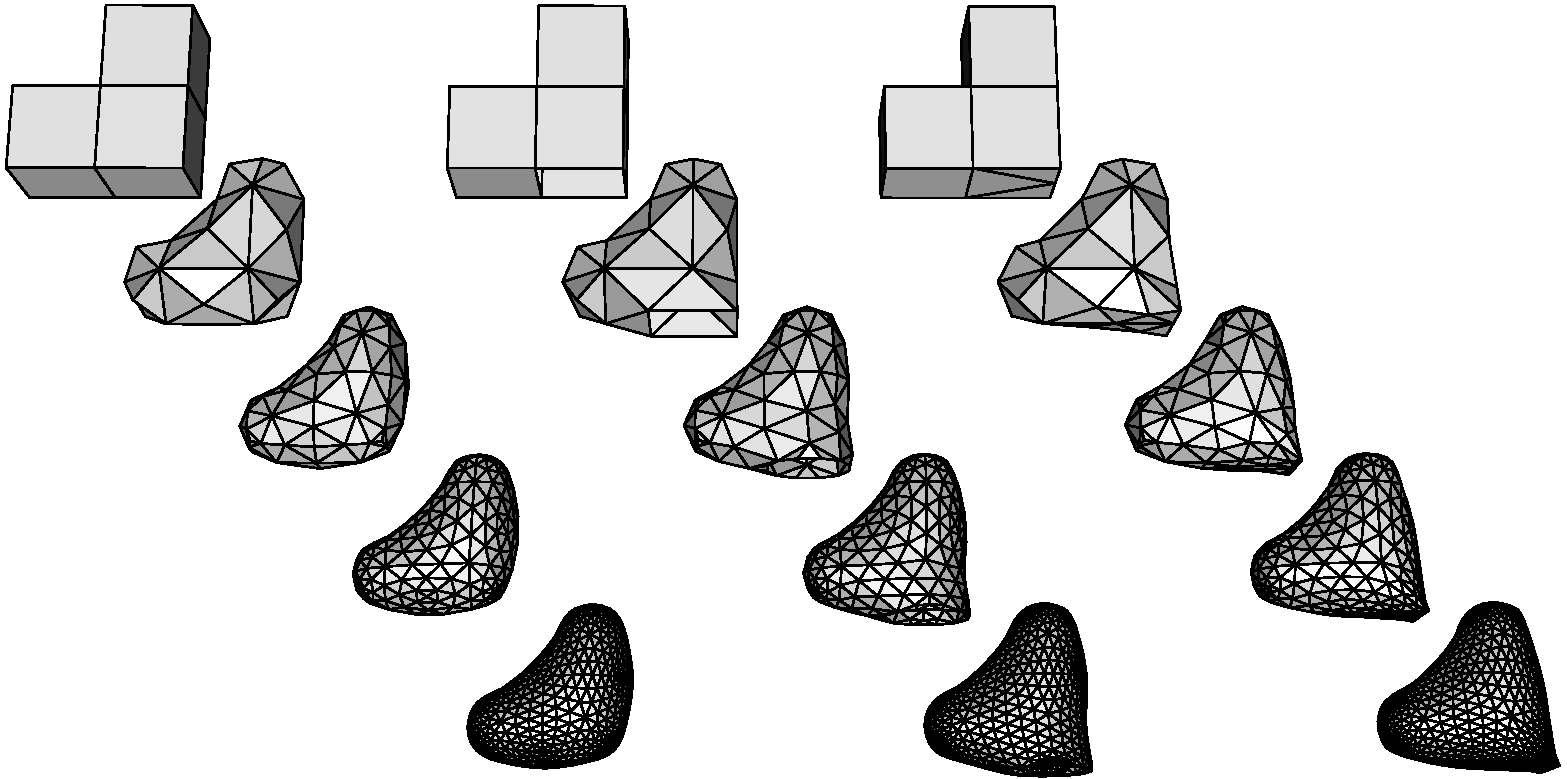
\includegraphics[width=\textwidth]{Polyhedron/fig/subdiv}%
      }
    \end{center}
\end{ccTexOnly}

\begin{ccHtmlOnly}
    <CENTER>
        <A HREF="./fig/subdiv.gif">
            <img src="./fig/subdiv_small.gif" alt="subdivision examples">
        </A><P>
    </CENTER>
\end{ccHtmlOnly}

The above figure shows three example objects, each 
subdivided four times. The initial object for the left sequence is
the closed surface of three unit cubes glued together to a corner.
The example program shown here can handle only closed surfaces, 
but the extended example
\texttt{examples/Polyhedron/polyhedron\_prog\_subdiv\_with\_boundary.cpp}
handles surfaces with boundary. So, the middle sequence starts with
the same surface where one of the facets has been removed. The boundary
subdivides to a nice circle. The third sequence creates a sharp
edge using a trick in the object presentation. The sharp edge is 
actually a hole whose vertex coordinates pinch the hole shut to form an
edge. The example directory \texttt{examples/Polyhedron/} contains the 
OFF files used here.

\ccIncludeExampleCode{Polyhedron/polyhedron_prog_subdiv.cpp}

% +------------------------------------------------------------------------+
\subsection{Example Using the Incremental Builder and Modifier Mechanism}

A utility class \ccc{CGAL::Polyhedron_incremental_builder_3} helps in
creating polyhedral surfaces from a list of points followed by a list
of facets that are represented as indices into the point list. This is
particularly useful for implementing file reader for common file
formats.  It is used here to create a triangle.

A modifier mechanism allows to access the internal representation of
the polyhedral surface, i.e., the halfedge data structure, in a
controlled manner. A modifier is basically a callback mechanism using
a function object. When called, the function object receives the
internal halfedge data structure as a parameter and can modify it.  On
return, the polyhedron can check the halfedge data structure for
validity. Such a modifier object must always return with a halfedge
data structure that is a valid polyhedral surface. The validity check is
implemented as an expensive postcondition at the end of the \ccc{delegate()}
member function, i.e., it is not called by default, only when expensive
checks are activated.

In this example, \ccc{Build_triangle} is such a function object
derived from \ccc{CGAL::Modifier_base<HalfedgeDS>}. The \ccc{delegate()}
member function of the polyhedron accepts this function object and calls
its \ccc{operator()} with a reference to its internally used halfedge 
data structure. Thus, this member function in \ccc{Build_triangle} can 
create the triangle in the halfedge data structure.

\ccIncludeExampleCode{Polyhedron/polyhedron_prog_incr_builder.cpp}

% +--------------------------------------------------------+

%% % =============================================================================
% The CGAL Reference Manual
% Chapter: Optimisation
% -----------------------------------------------------------------------------
% file  : doc_tex/basic/Optimisation/main.tex
% author: Bernd G�rtner, Sven Sch�nherr (sven@inf.fu-berlin.de)
% -----------------------------------------------------------------------------
% $Revision$
% $Date$
% =============================================================================

\newcommand{\linebreakByHand}{\ccTexHtml{\\}{}}
\newcommand{\SaveSpaceByHand}{}  %%%% [2]{\ccTexHtml{#1}{#2}}

\chapter{Geometric Optimisation} \label{Optimisation}
\RCSdefDate{\OptRCSDate}{$Date$}

\ccChapterRelease{Release: 2.0 \ccTexHtml{\quad}{ , } \OptRCSDate}

\ccChapterAuthor{Bernd G{\"a}rtner}\ccTexHtml{\\}{<br>}
\ccChapterAuthor{Michael Hoffmann}\ccTexHtml{\\}{<br>}
\ccChapterAuthor{Sven Sch{\"o}nherr}

\ccTexHtml{\thispagestyle{empty}}{}

\begin{ccTexOnly}\section*{Introduction}\end{ccTexOnly}
\begin{ccHtmlOnly}<H2>Introduction</H2><P>\end{ccHtmlOnly}

This chapter describes routines for solving geometric optimisation problems.
The first two sections contain algorithms for computing and updating the
smallest enclosing circle (Section~\ref{sec:smallest_enclosing_circles})
resp.\ ellipse (Section~\ref{sec:smallest_enclosing_ellipses}) of a finite
point set.  Formally, the `smallest enclosing circle' is the boundary of the
closed disk of minimum area covering the point set. It is known that this
disk is unique.  We usually identify the disk with its bounding circle,
allowing us to talk about points being on the boundary of the circle, etc.
The same holds for the smallest enclosing ellipse. These algorithms work in
an incremental manner. They are implemented as semi-dynamic data structures,
thus allowing to insert points while maintaining the smallest enclosing
circle resp.\ ellipse.

The remaining sections describe algorithms for searching in matrices with
specific properties and some applications. In particular, there are
general implementations of
\begin{itemize}
  \item monotone matrix search (see Section~\ref{secMonotoneMatrixSearch}),
    which can be applied to compute
    \begin{itemize}
      \item extremal polygons of a convex polygon
        (see Section~\ref{secComputingExtremalPolygons}) \textit{or}
      \item all furthest neighbors for the vertices of a convex polygon
        (see Section~\ref{secAllFurthestNeighbors}),
    \end{itemize}
  \item and sorted matrix search (see Section~\ref{secSortedMatrixSearch}),
    which can be used to compute the $p$-centers of a planar point set
    (see Section~\ref{sec_RectangularPCenters}).
\end{itemize}

\subsubsection*{Traits Class}
The class and function templates are parameterized with a traits class
which defines the abstract interface between the optimisation
algorithm and the primitives it uses. We provide traits class
implementations that interface the optimisation algorithms with the
\cgal\ kernel. For some algorithms, in addition, we provide traits
class adapters to user supplied point classes. Finally, we describe
the requirements that must be fulfilled by traits classes for
optimisation algorithms.  This is at the same time a specification for
using the provided traits class implementations as for users who want
to supply their own traits class.

\subsubsection*{Assertions}
The optimisation code uses infix \ccc{OPTIMISATION} in the assertions,
e.g.\ defining the compiler flag
\ccc{CGAL_OPTIMISATION_NO_PRECONDITIONS} switches precondition
checking off, cf.~Section~\ref{assertions}.

\newcommand{\cgalSetOptTraitsAdaptLayout}{\ccTexHtml{%
    \ccSetThreeColumns{CGAL_Oriented_side}{}{returns constants
      \ccc{CGAL_LEFTTURN}, \ccc{CGAL_COLLINEAR}}
    \ccPropagateThreeToTwoColumns}{}}
\newcommand{\cgalSetOptTraitsAdaptReqLayout}{\ccTexHtml{%
    \ccSetThreeColumns{CGAL_Oriented_side}{da.get_hw( Point p).}{}
    \ccPropagateThreeToTwoColumns}{}}

\newcommand{\cgalSetOptTraitsReqLayout}{\ccTexHtml{%
    \ccSetThreeColumns{CGAL_Oriented_side}{}{returns
      \ccc{CGAL_ON_BOUNDED_SIDE}, \ccc{CGAL_ON_BOUNDARY}}
    \ccPropagateThreeToTwoColumns}{}}

\ccHtmlNoClassToc

\input{smallest_enclosing_circles}

\input{smallest_enclosing_ellipses}

%% ==============================================================
%% Specification: Computing Extremal Polygons
%% --------------------------------------------------------------
%% file  : spec_extremal_polygons.awi
%% author: Michael Hoffmann
%% $Id$
%% ==============================================================

\clearpage
\section{Computing Extremal Polygons}
\label{secComputingExtremalPolygons}
\cgalColumnLayout

This section describes several functions to compute a maximal $k$-gon
$P_k$ that can be inscribed into a given convex polygon $P$. The
criterion for maximality can be chosen freely by defining an
appropriate traits class as specified in section
\ref{req_ExtremalPolygonTraits}. For \cgal\ point classes there are
two predefined traits classes to compute a maximum area (see section
\ref{secMaximumAreaInscribedKgon}) resp.  perimeter (see section
\ref{secMaximumPerimeterInscribedKgon}) inscribed $k$-gon.

\ccHtmlNoClassToc
\begin{ccHtmlClassFile}{computing_maximum_area_inscribed_k_gon.html}
  {Function Declaration of \ccc{maximum_area_inscribed_k_gon}}
  \ccHtmlNoClassIndex\ccHtmlNoClassLinks
  %% class wrapper to keep the font at a uniform size:
  \begin{ccClass}{dummy}
    \ccHtmlNoIndex\subsection{Computing a Maximum Area Inscribed $k$-gon}
  \label{secMaximumAreaInscribedKgon}
  \end{ccClass}
  
  This section describes a function to compute a maximal area $k$-gon
  $P_k$ that can be inscribed into a given convex polygon $P$. Note
  that $P_k$ is not unique in general, but it can be chosen in such a
  way that its vertices form a subset of the vertex set of $P$.

  \ccInclude{CGAL/extremal_polygon_2.h}

  \def\ccLongParamLayout{\ccTrue} 
  
  \ccGlobalFunction{
    template < class RandomAccessIC, class OutputIterator >
    OutputIterator
    maximum_area_inscribed_k_gon(
    RandomAccessIC points_begin,
    RandomAccessIC points_end,
    int k,
    OutputIterator o);}
  
  computes a maximum area inscribed $k$-gon of the convex polygon
  described by [\ccc{points_begin}, \ccc{points_end}), writes its
  vertices to \ccc{o} and returns the past-the-end iterator of this
  sequence.
  
  \ccHeading{Precondition}
  \begin{enumerate}
  \item Value type of \ccc{RandomAccessIC} has to be
    \ccc{Point_2<R>} for some representation class \ccc{R}.
  \item \ccc{OutputIterator} accepts the value type of
    \ccc{RandomAccessIC} as value type,
  \item the -- at least three -- points denoted by the range
    [\ccc{points_begin}, \ccc{points_end}) form the boundary of a convex
    polygon (oriented clock-- or counterclockwise) \textit{and}
  \item $k \ge 3$.
  \end{enumerate}

  \ccHeading{Note}
  
  On compilers not supporting member function templates, the parameter
  \ccc{RandomAccessIC} is fixed to \ccc{vector<Point_2>::iterator}
  where \ccc{Point_2} is the value type of \ccc{RandomAccessIC}.
  
  \ccImplementation The implementation uses monotone matrix
  search\cite{akmsw-gamsa-87} and has a worst case running time of $O(k
  \cdot n + n \cdot \log n)$, where $n$ is the number of vertices in
  $P$.

  \ccExample The following code generates a random convex polygon
  \ccc{p} with ten vertices and computes the maximum area inscribed
  five-gon of \ccc{p}.

  \ccIncludeVerbatim{extremal_polygon_2_example_area.C}

\end{ccHtmlClassFile}
    
\ccHtmlNoClassToc
\begin{ccHtmlClassFile}{computing_maximum_perimeter_inscribed_k_gon.html}
  {Function Declaration of \ccc{maximum_perimeter_inscribed_k_gon}}
  \ccHtmlNoClassIndex\ccHtmlNoClassLinks
  %% class wrapper to keep the font at a uniform size:
  \begin{ccClass}{dummy}
    \ccHtmlNoIndex\subsection{Computing a Maximum Perimeter Inscribed
      $k$-gon}
    \label{secMaximumPerimeterInscribedKgon}
  \end{ccClass}
  
  This section describes a function to compute a largest perimeter
  $k$-gon $P_k$ that can be inscribed in a given convex polygon $P$.
  Note that $P_k$ is not unique in general, but we know that its
  vertices form a subset of the vertex set of $P$.

  \ccInclude{CGAL/extremal_polygon_2.h}

  \def\ccLongParamLayout{\ccTrue}
  \ccGlobalFunction{
    template < class RandomAccessIC, class OutputIterator >
    OutputIterator
    maximum_perimeter_inscribed_k_gon(
    RandomAccessIC points_begin,
    RandomAccessIC points_end,
    int k,
    OutputIterator o);}
  
  computes a maximum perimeter inscribed $k$-gon of the convex polygon
  described by [\ccc{points_begin}, \ccc{points_end}), writes its
  vertices to \ccc{o} and returns the past-the-end iterator of this
  sequence.

  \ccHeading{Precondition}
  \begin{enumerate}
  \item Value type of \ccc{RandomAccessIC} has to be
    \ccc{Point_2<R>} for some representation class \ccc{R},
  \item there is a global function \ccc{R::FT sqrt( R::FT)}
    defined that computes the squareroot of a number,
  \item \ccc{OutputIterator} accepts the value type of
    \ccc{RandomAccessIC} as value type,
  \item the -- at least three -- points denoted by the range
    [\ccc{points_begin}, \ccc{points_end}) form the boundary of a
    convex polygon (oriented clock-- or counterclockwise) \textit{and}
  \item $k \ge 2$.
  \end{enumerate}

  \ccTagDefaults

  \ccHeading{Note}
  
  On compilers not supporting member function templates, the parameter
  \ccc{RandomAccessIC} is fixed to \ccc{vector<Point_2>::iterator}
  where \ccc{Point_2} is the value type of \ccc{RandomAccessIC}.
  
  \ccImplementation The implementation uses monotone matrix
  search\cite{akmsw-gamsa-87} and has a worst case running time of $O(k
  \cdot n + n \cdot \log n)$, where $n$ is the number of vertices in
  $P$.

  \ccExample The following code generates a random convex polygon
  \ccc{p} with ten vertices and computes the maximum perimeter inscribed
  five-gon of \ccc{p}.

  \ccIncludeVerbatim{extremal_polygon_2_example_perimeter.C}

\end{ccHtmlClassFile}

\begin{ccAdvanced}
  \ccHtmlNoClassToc
  \begin{ccHtmlClassFile}{computing_general_extremal_polygons.html}
    {Function Declaration of \ccc{extremal_polygon}}
    \ccHtmlNoClassIndex\ccHtmlNoClassLinks
    %% class wrapper to keep the font at a uniform size:
    \begin{ccClass}{dummy}
      \ccHtmlNoIndex\subsection{Computing General Extremal
        Polygons}\label{secGeneralExtremalPolygons}
    \end{ccClass}
    
    This section describes a general function to compute a maximal
    $k$-gon $P_k$ that can be inscribed in a given convex polygon $P$.
    The criterion for maximality and some basic operations have to
    specified in an appropriate traits class as specified in section
    \ref{req_ExtremalPolygonTraits}.
    
    \ccInclude{CGAL/extremal_polygons_2.h}

    \def\ccLongParamLayout{\ccTrue} 
    
    \ccGlobalFunction{
      template < class RandomAccessIC, class OutputIterator, class Traits >
      OutputIterator
      extremal_polygon(
      RandomAccessIC points_begin,
      RandomAccessIC points_end,
      int k,
      OutputIterator o,
      const Traits& t);}
    
    computes a maximal (as specified by \ccc{t}) inscribed $k$-gon of
    the convex polygon described by [\ccc{points_begin},
    \ccc{points_end}), writes its vertices to \ccc{o} and returns the
    past-the-end iterator of this sequence.
    
    \ccHeading{Precondition}
    \begin{enumerate}
    \item \ccc{Traits} has to satisfy the requirements stated in section
      \ref{req_ExtremalPolygonTraits},
    \item Value type of \ccc{RandomAccessIC} must be
      \ccc{Traits::Point_2},
    \item \ccc{OutputIterator} accepts \ccc{Traits::Point_2} as value
      type,
    \item the -- at least three -- points denoted by the range
      [\ccc{points_begin}, \ccc{points_end}) form the boundary of a
      convex polygon (oriented clock-- or counterclockwise) \textit{and}
    \item $k \ge \ccc{t.min_k()}$.
    \end{enumerate}
    
    \ccImplementation The implementation uses monotone matrix
    search\cite{akmsw-gamsa-87} and has a worst case running time of
    $O(k \cdot n + n \cdot \log n)$, where $n$ is the number of vertices
    in $P$.
  \end{ccHtmlClassFile}
  
  \ccHtmlNoClassToc\ccHtmlNoClassIndex\begin{ccClass}{Exp_traits}
    \ccCreationVariable{t}\ccTagFullDeclarations
    
    \subsection{Requirements for Extremal Polygon Traits
      Classes}\label{req_ExtremalPolygonTraits}
    
    \ccDefinition A class \ccClassName\ has to provide the following
    types and operations in order to qualify as a traits class for
    \ccc{extremal_polygon}.
    
    \ccTypes 
    
    \ccNestedType{Point_2}{class used for representing the input
      points.}
    
    \ccNestedType{FT}{class used for doing computations on point
      coordinates (has to fulfill field-type requirements).}
    
    \ccNestedType{Operation}{AdaptableBinaryFunction class \ccc{op}:
      \ccc{Point_2} $\times$ \ccc{Point_2} $\rightarrow$ \ccc{FT}.
      Together with \ccc{init} this operation recursively defines the
      objective function to maximize.  Let $p$ and $q$ be two vertices
      of a polygon $P$ such that $q$ precedes $p$ in the oriented
      vertex chain of $P$ starting with vertex $root$.  Then
      \ccc{op(p,q)} returns the value by which an arbitrary
      sub-polygon of $P$ with vertices from $[root,\, q]$ increases
      when $p$ is added to it. E.g. in the maximum area case this is
      the area of the triangle $(root,\, q,\, p)$.}

    \ccOperations
    
    \ccMemberFunction{int min_k() const;}{returns the minimal $k$ for
      which a maximal $k$-gon can be computed. (e.g. in the maximum
      area case this is three.)}
    
    \ccMemberFunction{FT init( const Point_2& p, const Point_2& q)
      const;}{returns the value of the objective function for a
      polygon consisting of the two points \ccc{p} and \ccc{q}. (e.g.
      in the maximum area case this is \ccc{FT( 0)}.)}
    
    \ccMemberFunction{Operation operation( const Point_2& p)
      const;}{return \ccc{Operation} where \ccc{p} is the fixed $root$
      point.}
    
    \ccMemberFunction{template < class RandomAccessIC, class
      OutputIterator > OutputIterator compute_min_k_gon(
      RandomAccessIC points_begin, RandomAccessIC points_end, FT&
      max_area, OutputIterator o) const;}{writes the points of
      [\ccc{points_begin}, \ccc{points_end}) forming a
      \ccc{min_k()}-gon rooted at \ccc{points_begin[0]} of maximal
      value to o and returns the past-the-end iterator for that
      sequence (== \ccc{o + min_k()}).}
    
    \ccMemberFunction{template < class RandomAccessIC > bool
      is_convex( RandomAccessIC points_begin, RandomAccessIC
      points_end) const;}{returns true, iff the points
      [\ccc{points_begin}, \ccc{points_end}) form a convex chain.}
    
    \ccHeading{Notes}
    \begin{itemize}
    \item \ccClassName\ccc{::is_convex} is only used for precondition
      checking. Therefore it needs not to be specified, in case that
      precondition checking is disabled.
    \item On compilers not supporting member function templates,
      \ccc{RandomAccessIC} is fixed to \ccc{vector<Point_2>::iterator}
      and \ccc{OutputIterator} is fixed to
      \ccc{vector<int>::reverse_iterator}.
      
    \end{itemize}
    
    \ccSeeAlso \ccInclude{CGAL/Extremal_polygon_traits_2.h}
    
    The classes \ccc{Kgon_area_traits<R>} and
    \ccc{Kgon_perimeter_traits<R>} (templatized with a \cgal\ 
    representation class) both fulfill these requirements.
    
  \end{ccClass}
\end{ccAdvanced}

%% --------------------------------------------------------------
%% EOF spec_extremal_polygons.awi
%% --------------------------------------------------------------

 
%% ==============================================================
%% Specification: All Furthest Neighbors
%% --------------------------------------------------------------
%% file  : spec_all_furthest_neighbors.awi
%% author: Michael Hoffmann
%% $Id$
%% ==============================================================

\cgalColumnLayout

\begin{ccRefFunction}{all_furthest_neighbors_2}
  
  \ccDefinition The function \ccRefName\ computes all furthest
  neighbors for the vertices of a convex polygon $P$, i.e. for each
  vertex $v$ of $P$ a vertex $f_v$ of $P$ such that the distance
  between $v$ and $f_v$ is maximized.

  \ccInclude{CGAL/all_furthest_neighbors_2.h}

  \def\ccLongParamLayout{\ccTrue} 
  
  \ccGlobalFunction{ template < class RandomAccessIC, class
    OutputIterator, class Traits > OutputIterator
    all_furthest_neighbors_2( RandomAccessIC points_begin,
    RandomAccessIC points_end, OutputIterator o, Traits t =
    Default_traits);}
  
  computes all furthest neighbors for the vertices of the convex
  polygon described by the range [\ccc{points_begin},
  \ccc{points_end}), writes their indices (relative to
  \ccc{points_begin}) to \ccc{o}\footnote{i.e. the furthest neighbor
    of \ccc{points_begin[}i\ccc{]} is \ccc{points_begin[}$i$-th number
    written to \ccc{o}\ccc{]}} and returns the past-the-end iterator
  of this sequence.
  
  \ccPrecond The points denoted by the non-empty range
  [\ccc{points_begin}, \ccc{points_end}) form the boundary of a convex
  polygon $P$ (oriented clock-- or counterclockwise).
  
  The geometric types and operations to be used for the computation
  are specified by the traits class parameter \ccc{t}. This parameter
  can be omitted if \ccc{RandomAccessIC} refers to a point type from
  the 2D-Kernel. In this case, a default traits class
  (\ccc{All_furthest_neighbors_default_traits_2<R>}) is used.
  
  \ccRequire
  \begin{enumerate}
  \item If \ccc{t} is specified explicitly, \ccc{Traits} is a model
    for \ccc{All_furthest_neighbors_traits_2}.
  \item Value type of \ccc{RandomAccessIC} is \ccc{Traits::Point_2} or
    -- if \ccc{t} is not specified explicitly -- \ccc{Point_2<R>} for
    some representation class \ccc{R}.
  \item \ccc{OutputIterator} accepts \ccc{int} as value type.
  \end{enumerate}
  
  \ccSeeAlso
  \ccRefIdfierPage{All_furthest_neighbors_traits_2}\\
  \ccRefIdfierPage{CGAL::All_furthest_neighbors_default_traits_2<R>}\\
  \ccRefIdfierPage{CGAL::monotone_matrix_search}
 
  \ccImplementation The implementation uses monotone matrix
  search\cite{akmsw-gamsa-87}. Its runtime complexity is linear in the
  number of vertices of $P$.
  
  \ccExample The following code generates a random convex polygon
  \ccc{p} with ten vertices, computes all furthest neighbors and
  writes the sequence of their indices (relative to
  \ccc{points_begin}) to \ccc{cout} (e.g. a sequence of
  \ccc{4788911224} means the furthest neighbor of
  \ccc{points_begin[0]} is \ccc{points_begin[4]}, the furthest
  neighbor of \ccc{points_begin[1]} is \ccc{points_begin[7]} etc.).
  
  \ccIncludeVerbatim{Optimisation_ref/all_furthest_neighbors_2_example_noheader.C}
\end{ccRefFunction}

\begin{ccRefClass}{All_furthest_neighbors_default_traits_2<R>}
  \ccCreationVariable{t}\ccTagFullDeclarations
  
  \ccDefinition The class \ccClassName\ provides the types and
  operations needed to compute all furthest neighbors for the vertices
  of a convex polygon.
  
  \ccRequirements
  The template parameter \ccc{R} is a model for \ccc{Kernel}.

  \ccIsModel 
  \ccRefIdfierPage{All_furthest_neighbors_traits_2}

  \ccTypes
  
  \ccNestedType{Point_2}{typedef to \ccc{R::Point_2}.}
  
  \ccNestedType{FT}{typedef to \ccc{R::FT}.}
  
  \ccNestedType{Distance}{AdaptableBinaryFunction class: \ccc{Point_2}
    $\times$ \ccc{Point_2} $\rightarrow$ \ccc{FT} computing the
    squared Euclidean distance between two points.}

  \ccOperations
  
  \ccMemberFunction{Distance distance_object();}{returns the
    function object for computing distances.}
  
  \ccMemberFunction{template < class RandomAccessIC > bool is_convex(
    RandomAccessIC points_begin, RandomAccessIC points_end)
    const;}{returns true, iff the points [\ccc{points_begin},
    \ccc{points_end}) form a convex chain.}
  
  \ccSeeAlso
  \ccRefIdfierPage{CGAL::all_furthest_neighbors_2}

  \ccHeading{Notes}
  \begin{itemize}
  \item \ccClassName\ccc{::is_convex} is used for precondition
    checking only.
  \end{itemize}
\end{ccRefClass}

\begin{ccRefConcept}{All_furthest_neighbors_traits_2}
  \ccCreationVariable{t}\ccTagFullDeclarations
  
  \ccDefinition The concept \ccRefName\ defines types and operations
  needed to compute all furthest neighbors for the vertices of a
  convex polygon using the function \ccc{all_furthest_neighbors_2}.
  
  \ccTypes
  
  \ccNestedType{Point_2}{class used for representing the input
    points.}
  
  \ccNestedType{FT}{class used for doing computations on point
    coordinates; it has to be a model for \ccc{FieldNumberType}.}
  
  \ccNestedType{Distance}{AdaptableBinaryFunction class: \ccc{Point_2}
    $\times$ \ccc{Point_2} $\rightarrow$ \ccc{FT} computing the
    squared Euclidean distance between two points.}

  \ccOperations
  
  \ccMemberFunction{Distance distance_object();}{returns the
    function object for computing distances.}
  
  \ccMemberFunction{template < class RandomAccessIC > bool is_convex(
    RandomAccessIC points_begin, RandomAccessIC points_end)
    const;}{returns true, iff the points [\ccc{points_begin},
    \ccc{points_end}) form a convex chain.}
  
  \ccHasModels 
  \ccRefIdfierPage{CGAL::All_furthest_neighbors_default_traits_2<R>}

  \ccSeeAlso
  \ccRefIdfierPage{CGAL::all_furthest_neighbors_2}

  \ccHeading{Notes}
  \begin{itemize}
  \item \ccClassName\ccc{::is_convex} is used for precondition
    checking only.
  \end{itemize}
\end{ccRefConcept}

%% --------------------------------------------------------------
%% EOF spec_all_furthest_neighbors.awi
%% --------------------------------------------------------------

 
%% ==============================================================
%% Specification: Rectangular p-Centers
%% --------------------------------------------------------------
%% file  : spec_rectangular_p_centers.awi
%% author: Michael Hoffmann
%% $Id$
%% ==============================================================

\cgalColumnLayout

\begin{ccRefFunction}{rectangular_p_center_2}
  \ccIndexMainItem[t]{rectilinear centers}
  \ccIndexMainItem[t]{rectangular centers}
  \ccIndexSubitem[t]{center}{rectangular}
  
  \ccDefinition The function \ccRefName\ computes rectilinear
  $p$-centers of a planar point set, i.e. a set of $p$ points such
  that the maximum minimal $L_{\infty}$-distance between both sets is
  minimized.
  
  More formally the problem can be defined as follows.
  
  \ccTexHtml{Given a finite set $\mathcal{P}$ of points, compute a
    point set $\mathcal{C}$ with $|\mathcal{C}| \le p$ such that the
    $p$-radius of $\mathcal{P}$,
    $$
    rad_p(\mathcal{P}) := \max_{P \in \mathcal{P}} \min_{Q \in
      \mathcal{C}} || P - Q ||_\infty
    $$
    is minimized. We can interpret $\mathcal{C}$ as the best
    approximation (with respect to the given metric) for $\mathcal{P}$
    with at most $p$ points.}{Given a finite set <IMG WIDTH=12
    HEIGHT=12 ALIGN=BOTTOM ALT="tex2html_wrap_inline17"
    SRC="./MatrixSearch_pcenter1.gif" > of points, compute a point set
    <IMG WIDTH=9 HEIGHT=13 ALIGN=BOTTOM ALT="tex2html_wrap_inline19"
    SRC="./MatrixSearch_pcenter2.gif" > with <IMG WIDTH=46 HEIGHT=24
    ALIGN=MIDDLE ALT="tex2html_wrap_inline21"
    SRC="./MatrixSearch_pcenter3.gif" > such that the <I>p</I>-radius
    of <IMG WIDTH=12 HEIGHT=12 ALIGN=BOTTOM
    ALT="tex2html_wrap_inline17" SRC="./MatrixSearch_pcenter1.gif" > ,
    <P> <IMG WIDTH=358 HEIGHT=24 ALIGN=BOTTOM ALT="displaymath27"
    SRC="./MatrixSearch_pcenter4.gif" > <P> is minimized. We can
    interpret <IMG WIDTH=9 HEIGHT=13 ALIGN=BOTTOM
    ALT="tex2html_wrap_inline19" SRC="./MatrixSearch_pcenter2.gif" >
    as the best approximation (with respect to the given metric) for
    <IMG WIDTH=12 HEIGHT=12 ALIGN=BOTTOM ALT="tex2html_wrap_inline17"
    SRC="./MatrixSearch_pcenter1.gif" > with at most <I>p</I> points.}

  \ccInclude{CGAL/rectangular_p_center_2.h}

  \def\ccLongParamLayout{\ccTrue} 
  
  \ccGlobalFunction{template < class ForwardIterator, class
    OutputIterator, class FT, class Traits > OutputIterator
    rectangular_p_center_2(ForwardIterator f, ForwardIterator l,
    OutputIterator o, FT& r, int p, const Traits& t =
    Default_traits);}
  
  computes rectilinear \ccc{p}-centers for the point set described by
  the range [\ccc{f}, \ccc{l}), sets \ccc{r} to the corresponding
  $p$-radius, writes the at most \ccc{p} center points to \ccc{o} and
  returns the past-the-end iterator of this sequence.
  
  \ccPrecond
  \begin{enumerate}
  \item The range [\ccc{f}, \ccc{l}) is not empty.
  \item 2 $\le$ \ccc{p} $\le$ 4.
  \end{enumerate}
  
  The geometric types and operations to be used for the computation
  are specified by the traits class parameter \ccc{t}. This parameter
  can be omitted if \ccc{ForwardIterator} refers to a point type from
  the 2D-Kernel. In this case, a default traits class
  (\ccc{Rectangular_p_center_default_traits_2<R>}) is used.
  
  \ccRequire
  \begin{enumerate}
  \item \textit{Either: (if no traits parameter is given)} Value type
    of \ccc{ForwardIterator} is \ccc{CGAL::Point_2<R>} for some
    representation class \ccc{R} and \ccc{FT} is equivalent to
    \ccc{R::FT},
  \item \textit{Or: (if a traits parameter is specified)} \ccc{Traits}
    is a model for \ccc{RectangularPCenterTraits_2}.
  \item \ccc{OutputIterator} accepts the value type of
    \ccc{ForwardIterator} as value type.
  \end{enumerate}  
  
  \ccSeeAlso
  \ccRefConceptPage{RectangularPCenterTraits_2}\\
  \ccRefIdfierPage{CGAL::Rectangular_p_center_default_traits_2<R>}\\
  \ccRefIdfierPage{CGAL::sorted_matrix_search}
  
  \ccImplementation The runtime is linear for $p \in \{2,\,3\}$ and
  $\mathcal{O}(n \cdot \log n)$ for $p = 4$ where $n$ is the number of
  input points. These runtimes are worst case optimal. The $3$-center
  algorithm uses a prune-and-search technique described in
  \cite{cgal:h-slacr-99}.  The $4$-center implementation uses sorted matrix
  search \cite{fj-fkppc-83,fj-gsrsm-84} and fast algorithms for
  piercing rectangles \cite{sw-rpppp-96}.
  
  \ccExample The following code generates a random set of ten points
  and computes its two-centers.

  \ccIncludeExampleCode{Matrix_search/rectangular_p_center_2_example_nohead.cpp}
\end{ccRefFunction}

\begin{ccRefClass}{Rectangular_p_center_default_traits_2<R>}
  \ccCreationVariable{t}\ccTagFullDeclarations
    
  \ccDefinition The class \ccRefName\ defines types and operations
  needed to compute rectilinear $p$-centers of a planar point set
  using the function \ccc{rectangular_p_center_2}.
  
  \ccRequirements The template parameter \ccc{R} is a model for
  \ccc{Kernel}.
  
  \ccIsModel
  \ccRefConceptPage{RectangularPCenterTraits_2}

  \ccTypes 
    
  \ccNestedType{FT}{typedef to \ccc{R::FT}.}
  
  \ccNestedType{Point_2}{typedef to \ccc{R::Point_2}.}
  
  \ccNestedType{Iso_rectangle_2}{typedef to \ccc{R::Iso_rectangle_2}.}
  
  \ccNestedType{Less_x_2}{typedef to \ccc{R::Less_x_2}.}
 
  \ccNestedType{Less_y_2}{typedef to \ccc{R::Less_y_2}.}
  
  \ccNestedType{Construct_vertex_2}{typedef to
    \ccc{R::Construct_vertex_2}.}
  
  \ccNestedType{Construct_iso_rectangle_2}{typedef to
    \ccc{R::Construct_iso_rectangle_2}.}
    
  \ccNestedType{Signed_x_distance_2}{adaptable binary function
    class: \ccc{Point_2} $\times$ \ccc{Point_2} $\rightarrow$
    \ccc{FT} returns the signed distance of two points'
    $x$-coordinates.}
  
  \ccNestedType{Signed_y_distance_2}{adaptable binary function
    class: \ccc{Point_2} $\times$ \ccc{Point_2} $\rightarrow$
    \ccc{FT} returns the signed distance of two points'
    $y$-coordinates.}
  
  \ccNestedType{Infinity_distance_2}{adaptable binary function
    class: \ccc{Point_2} $\times$ \ccc{Point_2} $\rightarrow$
    \ccc{FT} returns the $||\cdot||_{\infty}$ distance of two
    points.}
  
  \ccNestedType{Signed_infinity_distance_2}{adaptable binary
    function class: \ccc{Point_2} $\times$ \ccc{Point_2}
    $\rightarrow$ \ccc{FT} returns the signed $||\cdot||_{\infty}$
    distance of two points.}
  
  \ccNestedType{Construct_point_2_below_left_implicit_point_2}{
    3-argument function class: \ccc{Point_2} $\times$ \ccc{Point_2}
    $\times$ \ccc{FT} $\rightarrow$ \ccc{Point_2}. For arguments
    $(p,\,q,\,r)$ it returns the lower-left corner of the iso-oriented
    square with sidelength $r$ and upper-right corner at the
    intersection of the vertical line through $p$ and the horizontal
    line through $q$.}
    
  \ccNestedType{Construct_point_2_below_right_implicit_point_2}{
    3-argument function class: \ccc{Point_2} $\times$ \ccc{Point_2}
    $\times$ \ccc{FT} $\rightarrow$ \ccc{Point_2}. For arguments
    $(p,\,q,\,r)$ it returns the lower-right corner of the
    iso-oriented square with sidelength $r$ and upper-left corner at
    the intersection of the vertical line through $p$ and the
    horizontal line through $q$.}
    
  \ccNestedType{Construct_point_2_above_right_implicit_point_2}{
    3-argument function class: \ccc{Point_2} $\times$ \ccc{Point_2}
    $\times$ \ccc{FT} $\rightarrow$ \ccc{Point_2}. For arguments
    $(p,\,q,\,r)$ it returns the upper-right corner of the
    iso-oriented square with sidelength $r$ and lower-left corner at
    the intersection of the vertical line through $p$ and the
    horizontal line through $q$.}
    
  \ccNestedType{Construct_point_2_above_left_implicit_point_2}{
    3-argument function class: \ccc{Point_2} $\times$ \ccc{Point_2}
    $\times$ \ccc{FT} $\rightarrow$ \ccc{Point_2}. For arguments
    $(p,\,q,\,r)$ it returns the upper-left corner of the iso-oriented
    square with sidelength $r$ and lower-right corner at the
    intersection of the vertical line through $p$ and the horizontal
    line through $q$.}

  \ccOperations
  
  For every function class listed above there is a member function
  to fetch the corresponding function object.
  
  \ccMemberFunction{Inf_distance_2 inf_distance_2_object() const;}{}
  \ccGlue\ccMemberFunction{Signed_inf_distance_2
    signed_inf_distance_2_object() const;}{}
  
  \ccGlue\ccMemberFunction{Construct_vertex_2
    construct_vertex_2_object() const;}{}
  
  \ccGlue\ccMemberFunction{Construct_iso_rectangle_2
    construct_iso_rectangle_2_object() const;}{}
  
  \ccGlue\ccMemberFunction{Construct_iso_rectangle_2_below_left_point_2
    construct_iso_rectangle_2_below_left_point_2_object() const;}{}
  
  \ccGlue\ccMemberFunction{Construct_iso_rectangle_2_above_left_point_2
    construct_iso_rectangle_2_above_left_point_2_object() const;}{}
  
  \ccGlue\ccMemberFunction{Construct_iso_rectangle_2_below_right_point_2
    construct_iso_rectangle_2_below_right_point_2_object() const;}{}
  
  \ccGlue\ccMemberFunction{Construct_iso_rectangle_2_above_right_point_2
    construct_iso_rectangle_2_above_right_point_2_object() const;}{}
  
  \ccSeeAlso
  \ccRefIdfierPage{CGAL::rectangular_p_center_2}

\end{ccRefClass}

\begin{ccRefConcept}{RectangularPCenterTraits_2}
  \ccCreationVariable{t}\ccTagFullDeclarations
    
  \ccDefinition The concept \ccRefName\ defines types and operations
  needed to compute rectilinear $p$-centers of a planar point set
  using the function \ccc{rectangular_p_center_2}.
  
  \ccTypes 
    
  \ccNestedType{FT}{model for \ccRefConceptPage{FieldNumberType}.}
  
  \ccNestedType{Point_2}{model for
    \ccRefConceptPage{Kernel::Point_2}.}
  
  \ccNestedType{Iso_rectangle_2}{model for
    \ccRefConceptPage{Kernel::Iso_rectangle_2}.}
  
  \ccNestedType{Less_x_2}{model for
    \ccRefConceptPage{Kernel::Less_x_2}.}
  
  \ccNestedType{Less_y_2}{model for
    \ccRefConceptPage{Kernel::Less_y_2}.}
  
  \ccNestedType{Construct_vertex_2}{model for
    \ccRefConceptPage{Kernel::Construct_vertex_2}.}
  
  \ccNestedType{Construct_iso_rectangle_2}{model for
    \ccRefConceptPage{Kernel::Construct_iso_rectangle_2}.}
    
  \ccNestedType{Signed_x_distance_2}{adaptable binary function
    class: \ccc{Point_2} $\times$ \ccc{Point_2} $\rightarrow$
    \ccc{FT} returns the signed distance of two points'
    $x$-coordinates.}
  
  \ccNestedType{Signed_y_distance_2}{adaptable binary function
    class: \ccc{Point_2} $\times$ \ccc{Point_2} $\rightarrow$
    \ccc{FT} returns the signed distance of two points'
    $y$-coordinates.}
  
  \ccNestedType{Infinity_distance_2}{adaptable binary function
    class: \ccc{Point_2} $\times$ \ccc{Point_2} $\rightarrow$
    \ccc{FT} returns the $||\cdot||_{\infty}$ distance of two
    points.}
  
  \ccNestedType{Signed_infinity_distance_2}{adaptable binary
    function class: \ccc{Point_2} $\times$ \ccc{Point_2}
    $\rightarrow$ \ccc{FT} returns the signed $||\cdot||_{\infty}$
    distance of two points.}
  
  \ccNestedType{Construct_point_2_below_left_implicit_point_2}{
    3-argument function class: \ccc{Point_2} $\times$ \ccc{Point_2}
    $\times$ \ccc{FT} $\rightarrow$ \ccc{Point_2}. For arguments
    $(p,\,q,\,r)$ it returns the lower-left corner of the iso-oriented
    square with sidelength $r$ and upper-right corner at the
    intersection of the vertical line through $p$ and the horizontal
    line through $q$.}
    
  \ccNestedType{Construct_point_2_below_right_implicit_point_2}{
    3-argument function class: \ccc{Point_2} $\times$ \ccc{Point_2}
    $\times$ \ccc{FT} $\rightarrow$ \ccc{Point_2}. For arguments
    $(p,\,q,\,r)$ it returns the lower-right corner of the
    iso-oriented square with sidelength $r$ and upper-left corner at
    the intersection of the vertical line through $p$ and the
    horizontal line through $q$.}
    
  \ccNestedType{Construct_point_2_above_right_implicit_point_2}{
    3-argument function class: \ccc{Point_2} $\times$ \ccc{Point_2}
    $\times$ \ccc{FT} $\rightarrow$ \ccc{Point_2}. For arguments
    $(p,\,q,\,r)$ it returns the upper-right corner of the
    iso-oriented square with sidelength $r$ and lower-left corner at
    the intersection of the vertical line through $p$ and the
    horizontal line through $q$.}
    
  \ccNestedType{Construct_point_2_above_left_implicit_point_2}{
    3-argument function class: \ccc{Point_2} $\times$ \ccc{Point_2}
    $\times$ \ccc{FT} $\rightarrow$ \ccc{Point_2}. For arguments
    $(p,\,q,\,r)$ it returns the upper-left corner of the iso-oriented
    square with sidelength $r$ and lower-right corner at the
    intersection of the vertical line through $p$ and the horizontal
    line through $q$.}

  \ccOperations
  
  For every function class listed above there is a member function
  to fetch the corresponding function object.
  
  \ccMemberFunction{Inf_distance_2 inf_distance_2_object() const;}{}
  \ccGlue\ccMemberFunction{Signed_inf_distance_2
    signed_inf_distance_2_object() const;}{}
  
  \ccGlue\ccMemberFunction{Construct_vertex_2
    construct_vertex_2_object() const;}{}
  
  \ccGlue\ccMemberFunction{Construct_iso_rectangle_2
    construct_iso_rectangle_2_object() const;}{}
  
  \ccGlue\ccMemberFunction{Construct_iso_rectangle_2_below_left_point_2
    construct_iso_rectangle_2_below_left_point_2_object() const;}{}
  
  \ccGlue\ccMemberFunction{Construct_iso_rectangle_2_above_left_point_2
    construct_iso_rectangle_2_above_left_point_2_object() const;}{}
  
  \ccGlue\ccMemberFunction{Construct_iso_rectangle_2_below_right_point_2
    construct_iso_rectangle_2_below_right_point_2_object() const;}{}
  
  \ccGlue\ccMemberFunction{Construct_iso_rectangle_2_above_right_point_2
    construct_iso_rectangle_2_above_right_point_2_object() const;}{}
  
  \ccHasModels
  \ccRefIdfierPage{CGAL::Rectangular_p_center_default_traits_2<R>}

  \ccSeeAlso
  \ccRefIdfierPage{CGAL::rectangular_p_center_2}

\end{ccRefConcept}

%% --------------------------------------------------------------
%% EOF spec_rectangular_p_centers.awi
%% --------------------------------------------------------------

 
%% ==============================================================
%% Specification: Monotone Matrix Search
%% --------------------------------------------------------------
%% file  : spec_monotone_matrix_search.awi
%% author: Michael Hoffmann
%% $Id$
%% ==============================================================

\cgalColumnLayout

\begin{ccRefFunction}{monotone_matrix_search}
  \begin{ccAdvanced}
    
    \ccDefinition The function \ccRefName\ computes the maxima for all
    rows of a totally monotone matrix.
    
    More precisely, monotony for matrices is defined as follows.
    
    \ccTexHtml{Let $K$ be a totally ordered set, $M \in K^{(n,\, m)}$
      a matrix over $K$ and for $0 \le i < n$:
      $$
      rmax_M(i) :\in \left\{ \min_{0 \le j < m} j \: \left|\:
          M[i,\, j] = \max_{0 \le k < m} M[i,\, k] \right.\right\}
      $$
      the (leftmost) column containing the maximum entry in row
      $i$.  $M$ is called monotone, iff
      $$
      \forall\, 0 \le i_1 < i_2 < n\: :\: rmax_M(i_1) \le
      rmax_M(i_2)\; .
      $$
      $M$ is totally monotone, iff all of its submatrices are
      monotone (or equivalently: iff all $2 \times 2$ submatrices are
      monotone).}{Let <I>K</I> be a totally ordered set, <IMG WIDTH=84
      HEIGHT=31 ALIGN=MIDDLE ALT="tex2html_wrap_inline11"
      SRC="./MatrixSearch_totmon1.gif" > a matrix over <I>K</I> and
      for <IMG WIDTH=64 HEIGHT=24 ALIGN=MIDDLE
      ALT="tex2html_wrap_inline13" SRC="./MatrixSearch_totmon2.gif" >
      : <P> <IMG WIDTH=427 HEIGHT=39 ALIGN=BOTTOM ALT="displaymath15"
      SRC="./MatrixSearch_totmon3.gif" > <P> the (leftmost) column
      containing the maximum entry in row <I>i</I>.  <I>M</I> is
      called monotone, iff <P> <IMG WIDTH=411 HEIGHT=16 ALIGN=BOTTOM
      ALT="displaymath19" SRC="./MatrixSearch_totmon4.gif" > <P>
      <I>M</I> is totally monotone, iff all of its submatrices are
      monotone (or equivalently: iff all <IMG WIDTH=33 HEIGHT=20
      ALIGN=MIDDLE ALT="tex2html_wrap_inline21"
      SRC="./MatrixSearch_totmon5.gif" > submatrices are monotone).}
    
    \ccInclude{CGAL/monotone_matrix_search.h}

    \def\ccLongParamLayout{\ccTrue} 
    \ccTexHtml{%
      \ccSetThreeColumns{void}{}{\hspace*{8.5cm}}
      \ccPropagateThreeToTwoColumns}{}
    
    \ccGlobalFunction{template < class Matrix, class RandomAccessIC,
      class Compare_strictly > void monotone_matrix_search( const
      Matrix& m, RandomAccessIC t, const Compare_strictly&
      compare_strictly = less< Matrix::Value >());}
    
    computes the maximum (as specified by \ccc{compare_strictly})
    entry for each row of \ccc{m} and writes the corresponding column
    to \ccc{t}, i.e. \ccc{t[i]} is set to the index of the column
    containing the maximum element in row \ccc{i}. The maximum $m_r$
    of a row $r$ is the leftmost element for which
    \ccc{compare_strictly}$(m_r,\,x)$ is false for all elements $x$ in
    $r$.
    
    \cgalColumnLayout
    \ccPrecond \ccc{t} points to a structure of size at least
    \ccc{m.number_of_rows()}

    \ccRequire
    \begin{enumerate}
    \item \ccc{Matrix} is a model for
      \ccc{Monotone_matrix_search_traits}.
    \item Value type of \ccc{RandomAccessIC} is \ccc{int}.
    \item If \ccc{compare_strictly} is defined, it is an adaptable
      binary function: \ccc{Matrix::Value} $\times$
      \ccc{Matrix::Value} $\rightarrow$ \ccc{bool} describing a strict
      (non-reflexive) total ordering on \ccc{Matrix::Value}.
    \end{enumerate}
    
    \ccSeeAlso
    \ccRefIdfierPage{Monotone_matrix_search_traits}\\
    \ccRefIdfierPage{\ccPureGlobalScope all_furthest_neighbors_2}\\
    \ccRefIdfierPage{\ccPureGlobalScope maximum_area_inscribed_k_gon_2}\\
    \ccRefIdfierPage{\ccPureGlobalScope maximum_perimeter_inscribed_k_gon_2}\\
    \ccRefIdfierPage{\ccPureGlobalScope extremal_polygon_2}

    \ccImplementation The implementation uses an algorithm by Aggarwal
    et al.\cite{akmsw-gamsa-87}. The runtime is linear in the number
    of rows and columns of the matrix.

  \end{ccAdvanced}  
\end{ccRefFunction}

\begin{ccRefClass}{Dynamic_matrix<M>}
  \begin{ccAdvanced}
    \ccCreationVariable{d}\ccTagDefaults
    
    \ccDefinition The class \ccClassTemplateName\ is an adaptor for an
    arbitrary matrix class \ccc{M} to provide the dynamic operations
    needed for monotone matrix search.
    
    \ccRequirements \ccc{M} is a model for \ccc{Basic_matrix}.
    
    \ccInclude{CGAL/Dynamic_matrix.h}
    
    \ccIsModel
    \ccRefIdfierPage{Monotone_matrix_search_traits}\\
    \ccRefIdfierPage{Basic_matrix}

    \ccCreation
    
    \ccConstructor{Dynamic_matrix( const M& m);}{initializes
      \ccVar\ to \ccc{m}. \ccc{m} is \textit{not} copied, we only
      store a reference.}

    \ccOperations
    
    \ccMemberFunction{int number_of_columns() const;}{returns the
      number of columns.}
    
    \ccMemberFunction{int number_of_rows() const;}{returns the number
      of rows.}
    
    \ccMemberFunction{Entry operator()( int row, int column) const;}
    {returns the entry at position (\ccc{row}, \ccc{column}).
      \ccPrecond\\ $0 \le$ \ccc{row} $<$ \ccc{number_of_rows()} and\\ 
      $0 \le$ \ccc{column} $<$ \ccc{number_of_columns()}.}
    
    \ccMemberFunction{void replace_column( int old, int new);}{replace
      column \ccc{old} with column number \ccc{new}.  \ccPrecond\\ $0
      \le$ \ccc{old}, \ccc{new} $<$ \ccc{number_of_columns()}.}
    
    \ccMemberFunction{Matrix* extract_all_even_rows() const;}{returns
      a new Matrix consisting of all rows of \ccVar\ with even index,
      (i.e. first row is row $0$ of \ccVar, second row is row $2$ of
      \ccVar\ etc.). \ccPrecond \ccc{number_of_rows()} $> 0$.}
    
    \ccMemberFunction{void shrink_to_quadratic_size();}{deletes the
      rightmost columns, such that \ccVar\ becomes quadratic.
      \ccPrecond\\ \ccc{number_of_columns()} $\ge$
      \ccc{number_of_rows()}. \ccPostcond\\ \ccc{number_of_rows()}
      $==$ \ccc{number_of_columns()}.}
    
    \ccSeeAlso
    \ccRefIdfierPage{\ccPureGlobalScope monotone_matrix_search}\\
    \ccRefIdfierPage{Monotone_matrix_search_traits}\\
    \ccRefIdfierPage{Basic_matrix}

    \ccImplementation All operations take constant time except for
    \ccc{extract_all_even_rows} which needs time linear in the number
    of rows.
    
  \end{ccAdvanced}
\end{ccRefClass}

\begin{ccRefConcept}{Monotone_matrix_search_traits}
  \begin{ccAdvanced}
    \ccCreationVariable{m}\ccTagFullDeclarations
    
    \ccDefinition The concept \ccRefName\ is a refinement of
    \ccc{Basic_matrix} and defines types and operations needed to
    compute the maxima for all rows of a totally monotone matrix using
    the function \ccc{monotone_matrix_search}.
    
    \ccTypes
    
    \ccNestedType{Value}{The type of a matrix entry.}

    \ccOperations
    
    \ccMemberFunction{int number_of_columns() const;}{returns the
      number of columns.}
    
    \ccMemberFunction{int number_of_rows() const;}{returns the number
      of rows.}
    
    \ccMemberFunction{Entry operator()( int row, int column) const;}
    {returns the entry at position (\ccc{row}, \ccc{column}).
      \ccPrecond\\ $0 \le$ \ccc{row} $<$ \ccc{number_of_rows()} and\\
      $0 \le$ \ccc{column} $<$ \ccc{number_of_columns()}.}
    
    \ccMemberFunction{void replace_column( int old, int new);}{replace
      column \ccc{old} with column number \ccc{new}.  \ccPrecond\\ $0
      \le$ \ccc{old}, \ccc{new} $<$ \ccc{number_of_columns()}.}
    
    \ccMemberFunction{Matrix* extract_all_even_rows() const;}{returns
      a new Matrix consisting of all rows of \ccVar\ with even index,
      (i.e. first row is row $0$ of \ccVar, second row is row $2$ of
      \ccVar\ etc.). \ccPrecond \ccc{number_of_rows()} $> 0$.}
    
    \ccMemberFunction{void shrink_to_quadratic_size();}{deletes the
      rightmost columns, such that \ccVar\ becomes quadratic.
      \ccPrecond\\ \ccc{number_of_columns()} $\ge$
      \ccc{number_of_rows()}. \ccPostcond\\ \ccc{number_of_rows()} $==$
      \ccc{number_of_columns()}.}
    
    \ccHeading{Notes}
    \begin{itemize}
    \item For the sake of efficiency (and in order to achieve the time
      bounds claimed for \ccc{monotone_matrix_search}), all these
      operations have to be realized in constant time -- except for
      \ccc{extract_all_even_rows} which may take linear time.
    \item There is an adaptor \ccc{Dynamic_matrix} that can be used to
      add most of the functionality described above to arbitrary
      matrix classes.
    \end{itemize}
    
    \ccHasModels
    \ccRefIdfierPage{\ccPureGlobalScope Dynamic_matrix<M>}

    \ccSeeAlso
    \ccRefIdfierPage{\ccPureGlobalScope monotone_matrix_search}

  \end{ccAdvanced}
\end{ccRefConcept}

\begin{ccRefConcept}{Basic_matrix}
  \begin{ccAdvanced}
    \ccCreationVariable{m}\ccTagFullDeclarations
    
    \ccDefinition A class \ccClassName\ has to provide the following
    types and operations in order to be a model for
    \ccc{Basic_matrix}.
    
    \ccTypes
    
    \ccNestedType{Value}{The type of a matrix entry. It has to define
      a copy constructor.}
    
    \ccOperations
    
    \ccMemberFunction{int number_of_columns() const;}{returns the
      number of columns.}
    
    \ccMemberFunction{int number_of_rows() const;}{returns the
      number of rows.}
    
    \ccMemberFunction{Entry operator()( int row, int column) const;}
    {returns the entry at position (\ccc{row}, \ccc{column}).
      \ccPrecond\\ $0 \le$ \ccc{row} $<$ \ccc{number_of_rows()} and\\
      $0 \le$ \ccc{column} $<$ \ccc{number_of_columns()}.}

    \ccHasModels
    \ccRefIdfierPage{\ccPureGlobalScope Dynamic_matrix<M>}

    \ccSeeAlso
    \ccRefIdfierPage{Monotone_matrix_search_traits}\\
    \ccRefIdfierPage{Sorted_matrix_search_traits}
    
  \end{ccAdvanced}
\end{ccRefConcept}

%% --------------------------------------------------------------
%% EOF spec_monotone_matrix_search.awi
%% --------------------------------------------------------------

 
%% ==============================================================
%% Specification: Sorted Matrix Search
%% --------------------------------------------------------------
%% file  : spec_sorted_matrix_search.awi
%% author: Michael Hoffmann
%% $Id$
%% ==============================================================

\cgalColumnLayout
  
\begin{ccRefFunction}{sorted_matrix_search}
  \ccIndexMainItem[t]{sorted matrix search}
  \ccIndexSubitem[t]{searching}{in sorted matrices}
  \ccIndexSubitem[t]{matrix}{sorted}
  \ccIndexSubitem[t]{matrix}{searching}
  \ccIndexMainItem[t]{Frederickson/Johnson matrix search}
  
  \begin{ccAdvanced}
    \ccDefinition The function \ccRefName\ selects the smallest entry
    in a set of sorted matrices that fulfills a certain feasibility
    criterion.
    
    \ccTexHtml{More exactly, a matrix $M = (m_{i j}) \in S^{r \times
        l}$ (over a totally ordered set $S$) is sorted, iff
      \begin{eqnarray*}
        \forall \, 1 \le i \le r,\; 1 \le j < l\; :\; m_{i j} \le m_{i (j+1)} 
        \;\; {\it and}\\ 
        \forall \, 1 \le i < r,\; 1 \le j \le l\; :\; m_{i j} \le m_{(i+1) j} 
        \;\;.
      \end{eqnarray*}
      
      Now let $\mathcal{M}$ be a set of $n$ sorted matrices over $S$
      and $f$ be a monotone predicate on $S$, i.e.
      $$
      f\: :\: S \longrightarrow\, \textit{bool} \quad{\rm with}\quad f(r)
      \;\Longrightarrow\; \forall\, t \in S\,,\: t > r \; :\; f(t)\;.
      $$}{More exactly, a matrix <IMG WIDTH=124 HEIGHT=30 ALIGN=MIDDLE
      ALT="tex2html_wrap_inline18" SRC="./MatrixSearch_sorted1.gif" >
      (over a totally ordered set <I>S</I>) is sorted, iff <P> <IMG
      WIDTH=500 HEIGHT=41 ALIGN=BOTTOM ALT="eqnarray5"
      SRC="./MatrixSearch_sorted2.gif" > <P> <P> Now let <IMG WIDTH=18
      HEIGHT=13 ALIGN=BOTTOM ALT="tex2html_wrap_inline22"
      SRC="./MatrixSearch_sorted3.gif" > be a set of <I>n</I> sorted
      matrices over <I>S</I> and <I>f</I> be a monotone predicate on
      <I>S</I>, i.e.  <P> <IMG WIDTH=445 HEIGHT=16 ALIGN=BOTTOM
      ALT="displaymath32" SRC="./MatrixSearch_sorted4.gif" > <P><BR>}
    
    If we assume there is any feasible element in one of the matrices
    in \ccTexHtml{$\mathcal{M}$}{<IMG WIDTH=18 HEIGHT=13 ALIGN=BOTTOM
      ALT="tex2html_wrap_inline21" SRC="./MatrixSearch_sorted3.gif"
      >}, there certainly is a smallest such element. This is the one
    we are searching for.
    
    The feasibility test as well as some other parameters can (and
    have to) be customized through a traits class. 
    
    \ccInclude{CGAL/sorted_matrix_search.h}

    \def\ccLongParamLayout{\ccTrue} 
    
    \ccGlobalFunction{template < class RandomAccessIC, class Traits >
      Traits::Value sorted_matrix_search( RandomAccessIC f,
      RandomAccessIC l, const Traits& t);}

    returns the element \ccc{x} in one of the sorted matrices from the
    range $\left[ f,\, l \right)$, for which \ccc{t.is_feasible( x)}
    is true and \ccc{t.compare( x, y)} is true for all other
    \ccc{y} values from any matrix for which \ccc{t.is_feasible(
      y)} is true.
    
    \ccPrecond
    \begin{enumerate}
    \item All matrices in $\left[f,\, l\right)$ are sorted according
      to \ccc{Traits::compare_non_strictly}.
    \item There is at least one entry $x$ in a matrix $M \in
      \left[f,\, l\right)$ for which \ccc{Traits::is_feasible(x)} is
      true.
    \end{enumerate}
    
    \ccRequire
    \begin{enumerate}
    \item \ccc{Traits} is a model for
      \ccc{Sorted_matrix_search_traits}.
    \item Value type of \ccc{RandomAccessIC} is \ccc{Traits::Matrix}.
    \end{enumerate}
    
    \ccSeeAlso
    \ccRefConceptPage{Sorted_matrix_search_traits}
    
    \ccImplementation The implementation uses an algorithm by
    Frederickson and Johnson\cite{fj-fkppc-83,fj-gsrsm-84} and runs in
    $\mathcal{O}(n \cdot k + f \cdot \log (n \cdot k))$, where $n$ is
    the number of input matrices, $k$ denotes the maximal dimension of
    any input matrix and $f$ the time needed for one feasibility test.
    
    \ccExample In the following program we build a random vector $a =
    (a_i)_{i = 1,\,\ldots,\,5}$ (elements drawn uniformly from $\{
    0,\,\ldots,\,99 \}$) and construct a Cartesian matrix $M$
    containing as elements all sums $a_i + a_j,\: i,\,j \in
    \{1,\,\ldots,\,5\}$. If $a$ is sorted, $M$ is sorted as well. So
    we can apply \ccc{sorted_matrix_search} to compute the upper bound
    for the maximal entry of $a$ in $M$.
    
    \ccIncludeVerbatim{Optimisation_ref/sorted_matrix_search_example_noheader.C}

  \end{ccAdvanced}
\end{ccRefFunction}

\begin{ccRefClass}{Sorted_matrix_search_traits_adaptor<F,M>}
  \begin{ccAdvanced}
    \ccCreationVariable{t}\ccTagFullDeclarations
    
    \ccInclude{CGAL/Sorted_matrix_search_traits_adaptor.h}
    
    \ccDefinition The class \ccClassTemplateName\ can be used as an
    adaptor to create sorted matrix search traits classes for
    arbitrary feasibility test and matrix classes \ccc{F} resp.
    \ccc{M}.

    \ccIsModel
    \ccRefConceptPage{Sorted_matrix_search_traits}
    
    \ccRequirements

    \begin{enumerate}
    \item \ccc{M} is a model for \ccc{Basic_matrix} \textit{and}
    \item \ccc{F} defines a copy constructor and a monotone \ccc{bool
        operator()( const Value&)}.
    \end{enumerate}

    \ccCreation
    
    \ccConstructor{Sorted_matrix_search_traits_adaptor<F,M>( const F&
      m);}{initializes \ccVar\ to use \ccc{m} for feasibility
      testing.}
    
    \ccTypes 
    
    \ccNestedType{Matrix}{typedef to \ccc{M}.}
    
    \ccNestedType{Value}{typedef to \ccc{Matrix::Value}.}
    
    \ccNestedType{Compare_strictly}{typedef to
      \ccc{std::less<Value>}.}
    
    \ccNestedType{Compare_non_strictly}{typedef to
      \ccc{std::less_equal<Value>}.}

    \ccOperations
    
    \ccMemberFunction{Compare_strictly compare_strictly()
      const;}{returns the \ccc{Compare_strictly} object to be used for
      the search.}
    
    \ccMemberFunction{Compare_non_strictly compare_non_strictly()
      const;}{returns the \ccc{Compare_non_strictly} object to be used
      for the search.}
    
    \ccMemberFunction{bool is_feasible(const Value& a);}{uses the
      feasibility test given during creation.}

    \ccTagDefaults
  \end{ccAdvanced}
\end{ccRefClass}

\begin{ccRefConcept}{Sorted_matrix_search_traits}
  \begin{ccAdvanced}
    \ccCreationVariable{t}\ccTagFullDeclarations
    
    \ccDefinition The concept \ccRefName\ defines types and operations
    needed to compute the smallest entry in a set of sorted matrices
    that fulfills a certain feasibility criterion using the function
    \ccc{sorted_matrix_search}.
    
    \ccTypes 
    
    \ccNestedType{Matrix}{The class used for representing matrices.
      It has to be a model for \ccc{Basic_matrix}.}

    \ccTypedef{typedef Matrix::Value Value;}{The class used for
      representing the matrix elements.}
    
    \ccNestedType{Compare_strictly}{An adaptable binary function
      class: \ccc{Value} $\times$ \ccc{Value} $\rightarrow$ \ccc{bool}
      defining a non-reflexive total order on \ccc{Value}. This
      determines the direction of the search.}
    
    \ccNestedType{Compare_non_strictly}{An adaptable binary function
      class: \ccc{Value} $\times$ \ccc{Value} $\rightarrow$ \ccc{bool}
      defining the reflexive total order on \ccc{Value} corresponding
      to \ccc{Compare_strictly}.}

    \ccOperations
    
    \ccMemberFunction{Compare_strictly compare_strictly()
      const;}{returns the \ccc{Compare_strictly} object to be used for
      the search.}
    
    \ccMemberFunction{Compare_non_strictly compare_non_strictly()
      const;}{returns the \ccc{Compare_non_strictly} object to be used
      for the search.}
    
    \ccMemberFunction{bool is_feasible( const Value& a);}{The
      predicate to determine whether an element \ccc{a} is feasible.
      It has to be monotone in the sense that \ccc{compare( a, b)} and
      \ccc{is_feasible( a)} imply \ccc{is_feasible( b)}.}

    \ccHasModels
    \ccRefIdfierPage{CGAL::Sorted_matrix_search_traits_adaptor<F,M>}
    
    \ccSeeAlso
    \ccRefIdfierPage{CGAL::sorted_matrix_search}\\
    \ccRefConceptPage{Basic_matrix}
    
    \ccTagDefaults
  \end{ccAdvanced}
\end{ccRefConcept}
  
%% --------------------------------------------------------------
%% EOF spec_sorted_matrix_search.awi
%% --------------------------------------------------------------


% ===== EOF ===================================================================


% EOF


